%%%%%%%%%%%%%%%%%%%%%%%%%%%%%%%%%%%%%%%%%%%%%%%%%%%%%%%%%%%%%%%%%%%%%%
% Template for a UBC-compliant dissertation
% At the minimum, you will need to change the information found
% after the "Document meta-data"
%
%!TEX TS-program = pdflatex
%!TEX encoding = UTF-8 Unicode

%% The ubcdiss class provides several options:
%%   gpscopy (aka fogscopy)
%%       set parameters to exactly how GPS specifies
%%         * single-sided
%%         * page-numbering starts from title page
%%         * the lists of figures and tables have each entry prefixed
%%           with 'Figure' or 'Table'
%%       This can be tested by `\ifgpscopy ... \else ... \fi'
%%   10pt, 11pt, 12pt
%%       set default font size
%%   oneside, twoside
%%       whether to format for single-sided or double-sided printing
%%   balanced
%%       when double-sided, ensure page content is centred
%%       rather than slightly offset (the default)
%%   singlespacing, onehalfspacing, doublespacing
%%       set default inter-line text spacing; the ubcdiss class
%%       provides \textspacing to revert to this configured spacing
%%   draft
%%       disable more intenssdive processing, such as including
%%       graphics, etc.
%%

% For submission to GPS
\documentclass[gpscopy,onehalfspacing,11pt]{ubcdiss}
\usepackage[margin=1in,
			left=1.1in]{geometry}
\makeatother


%!TEX root = MJThesis.tex
%%%%%%%%%%%%%%%%%%%%%%%%%%%%%%%%%%%%%%%%%%%%%%%%%%%%%____FONTS___%%%%%
%%
%% FONTS:
%% 
%% The defaults below configures Times Roman for the serif font,
%% Helvetica for the sans serif font, and Courier for the
%% typewriter-style font.  Configuring fonts can be time
%% consuming; we recommend skipping to END FONTS!
%% 
%% If you're feeling brave, have lots of time, and wish to use one
%% your platform's native fonts, see the commented out bits below for
%% XeTeX/XeLaTeX.  This is not for the faint at heart. 
%% (And shouldn't you be writing? :-)
%%

%% NFSS font specification (New Font Selection Scheme)
\usepackage{times,mathptmx,courier}
\usepackage[scaled=.92]{helvet}
\usepackage{sectsty}
\chapterfont{\usefont{T1}{qhv}{b}{n}\selectfont\huge}
%% Math or theory people may want to include the handy AMS macros
%\usepackage{amssymb}
%\usepackage{amsmath}
%\usepackage{amsfonts}
\usepackage{pifont, fixltx2e} % Adds \textsubscript{}, at least
\usepackage{titlesec} % titles! 
\usepackage{mhchem} % chemistry! \ce ;chem
\usepackage{float} % Floats! Now can use H as a placement option on floats.
\titleformat{\section}[hang]{
    \usefont{T1}{qhv}{b}{n}\selectfont} % "qhv" - TeX Gyre Heros, "b" - bold
    {} 
    {0em}
    {\hspace{-0.4pt}\Large \thesection\hspace{0.6em}}

%%%%%%%%%%%%%%%%%%%%%%%%%%%%%%%%%%%%%%%%%%%%%%%%%%%%%%____TOC___%%%%%
\usepackage{tocloft} % subfigure option only if using subfigure package
\renewcommand{\cfttoctitlefont} % ToC title
             {\usefont{T1}{qhv}{b}{n}\selectfont\huge}
\renewcommand{\cftchapfont} % chapter titles
             {\usefont{T1}{qhv}{b}{n}\selectfont}
\renewcommand{\cftsecfont} % section titles
             {\usefont{T1}{bch}{m}{n}\selectfont}
\renewcommand{\cftsubsecfont} % subsection titles
             {\usefont{T1}{bch}{m}{n}\selectfont} 
\renewcommand{\cftchappagefont} % chapter page numbers
             {\usefont{T1}{bch}{b}{n}\selectfont}
\renewcommand{\cftsecpagefont} % section page numbers
             {\cftsecfont} 
\renewcommand{\cftsubsecpagefont} % subsection page numbers
             {\cftsubsecfont}
%%%%%%%%%%%%%%%%%%%%%%%%%%%%%%%%%%%%%%%%%%%%%%%%____MICROTYPE___%%%%%
\usepackage[activate={true,nocompatibility},final,tracking=true,kerning=true,spacing=true,factor=1100,stretch=10,shrink=10]{microtype}
% activate={true,nocompatibility} - activate protrusion and expansion
% final - enable microtype; use "draft" to disable
% tracking=true, kerning=true, spacing=true - activate these techniques
% factor=1100 - add 10% to the protrusion amount (default is 1000)
% stretch=10, shrink=10 - reduce stretchability/shrinkability (default is 20/20)
\SetProtrusion{encoding={*},family={bch},series={*},size={6,7}}
              {1={ ,750},2={ ,500},3={ ,500},4={ ,500},5={ ,500},
               6={ ,500},7={ ,600},8={ ,500},9={ ,500},0={ ,500}}
\SetExtraKerning[unit=space]
    {encoding={*}, family={bch}, series={*}, size={footnotesize,small,normalsize}}
    {\textendash={400,400}, % en-dash, add more space around it
     "28={ ,150}, % left bracket, add space from right
     "29={150, }, % right bracket, add space from left
     \textquotedblleft={ ,150}, % left quotation mark, space from right
     \textquotedblright={150, }} % right quotation mark, space from left
\SetExtraKerning[unit=space]
   {encoding={*}, family={qhv}, series={b}, size={large,Large}}
   {1={-200,-200}, 
    \textendash={400,400}}
\SetTracking{encoding={*}, shape=sc}{20}   
\microtypecontext{spacing=nonfrench}        
%%%%%%%%%%%%%%%%%%%%%%%%%%%%%%%%%%%%%%%%%%%%%%%%%%%%%%%%%%%%%%%%%%%%%%
%%
%% Recommended packages
%%
\usepackage{checkend}	% better error messages on left-open environments
\usepackage{graphicx}	% for incorporating external images

%% booktabs: provides some special commands for typesetting tables as used
%% in excellent journals.  Ignore the examples in the Lamport book!
\usepackage{booktabs, multirow}
\usepackage{siunitx, xspace} %for SI units eg. \si{\grams\per\mega\hertz} and gives xspace

%% The acronym package provides support for defining acronyms, providing
%% their expansion when first used, and building glossaries.  See the
%% example in glossary.tex and the example usage throughout the example
%% document.
%% NOTE: to use \MakeTextLowercase in the \acsfont command below,
%%   we *must* use the `nohyperlinks' option -- it causes errors with
%%   hyperref otherwise.  See Section 5.2 in the ``LaTeX 2e for Class
%%   and Package Writers Guide'' (clsguide.pdf) for details.
\usepackage[printonlyused,nohyperlinks]{acronym}
%% The ubcdiss.cls loads the `textcase' package which provides commands
%% for upper-casing and lower-casing text.  The following causes
%% the acronym package to typeset acronyms in small-caps
%% as recommended by Bringhurst.
\renewcommand{\acsfont}[1]{{\scshape \MakeTextLowercase{#1}}}

%% color: add support for expressing colour models.  Grey can be used
%% to great effect to emphasize other parts of a graphic or text.
%% For an excellent set of examples, see Tufte's "Visual Display of
%% Quantitative Information" or "Envisioning Information".
\usepackage{color}
\definecolor{greytext}{gray}{0.5}
%%%%%%%%%%%%%%%%%%%%%%%%%%%%%%%%%%%%%%%%%%%%%%%%%%____COMMENT___%%%%%
%% comment: provides a new {comment} environment: all text inside the
%% environment is ignored.
%%   \begin{comment} ignored text ... \end{comment}
\usepackage{comment}

\titleformat*{\section}{\singlespacing\raggedright\bfseries\Large}
\titleformat*{\subsection}{\singlespacing\raggedright\bfseries\large}
\titleformat*{\subsubsection}{\singlespacing\raggedright\bfseries}
\titleformat*{\paragraph}{\singlespacing\raggedright\itshape}
%%%%%%%%%%%%%%%%%%%%%%%%%%%%%%%%%%%%%%%%%%%%%%%%%%____CAPTION___%%%%%
%% The caption package provides support for varying how table and
%% figure captions are typeset.
\usepackage[format=hang,indention=-1cm,labelfont={bf},margin=1em]{caption}

%% url: for typesetting URLs and smart(er) hyphenation.
%% \url{http://...} 
\usepackage{url}
\urlstyle{sf}	% typeset urls in sans-serif

%!TEX root = MJThesis.tex
%%%%%%%%%%%%%%%%%%%%%%%%%%%%%%%%%%%%%%%%%%%%%%%%%%%%%%%%%%%%%%%%%%%%%%
%% HYPERREF:
%% The hyperref package provides for embedding hyperlinks into your
%% document.  By default the table of contents, references, citations,
%% and footnotes are hyperlinked.
%%
%% Hyperref provides a very handy command for doing cross-references:
%% \autoref{}.  This is similar to \ref{} and \pageref{} except that
%% it automagically puts in the *type* of reference.  For example,
%% referencing a figure's label will put the text `Figure 3.4'.
%% And the text will be hyperlinked to the appropriate place in the
%% document.
%%
%% Generally hyperref should appear after most other packages

%% The following puts hyperlinks in very faint grey boxes.
%% The `pagebackref' causes the references in the bibliography to have
%% back-references to the citing page; `backref' puts the citing section
%% number.  See further below for other examples of using hyperref.
%% 2009/12/09: now use `linktocpage' (Jacek Kisynski): GPS now prefers
%%   that the ToC, LoF, LoT place the hyperlink on the page number,
%%   rather than the entry text.
%% The following is a directive for TeXShop to indicate the main file

\usepackage[hyperref=true,
            url=false,
            isbn=false,
            backref=true,
            style=custom-numeric-comp,
            citereset=chapter,
            maxcitenames=3,
            maxbibnames=100,
            backend=bibtex, % while checking on one of my (newest) systems, this option was needed to generate bibliography
            block=none]{biblatex}

    \usepackage{varioref}

    \usepackage[
		    bookmarksopen=true,
		    linktocpage=true,
		    urlcolor=linkcolor, % Color of URLs
		    citecolor=linkcolor, % Color of citations
		    linkcolor=linkcolor, % Color of links to other pages/figures
		    % backref=page,
		    pdfpagelabels=true,
		    plainpages=false,
		    % colorlinks=true, % Turn off all coloring by changing this to false
		    bookmarks=true,
		    pdfview=FitB]{hyperref}

		    %% The following change how the the back-references text is typeset in a
		    %% bibliography when `backref' or `pagebackref' are used
		    % \renewcommand\backrefpagesname{\(\rightarrow\) pages}
		    % \renewcommand\backref{\textcolor{greytext} \backrefpagesname\ }
    %%%%%%%%%%%%%%%%%%%%%%%%%%%%%%
    % Customisation
    %%%%%%%%%%%%%%%%%%%%%%%%%%%%%%
    % back reference text preceding the page number ("see p.")
    \DefineBibliographyStrings{english}{%
        backrefpage  = {see p.}, % for single page number
        backrefpages = {see pp.} % for multiple page numbers
    }

    % the followings activate 'custom-english-ordinal-sscript.lbx'
    % in order to print ordinal 'edition' suffixes as superscripts,
    % and adjusts (reduces) spacing between suffix and following "ed."
    \DeclareLanguageMapping{english}{custom-english-ordinal-sscript}
    \DeclareFieldFormat{edition}%
                       {\ifinteger{#1}%
                        {\mkbibordedition{#1}\addthinspace{}ed.}%
                        {#1\isdot}}

    % removes period at the very end of bibliographic record
    \renewcommand{\finentrypunct}{}

    % removes period after DOI and suppresses capitalization
    % of the word following DOI ("See p. xx" -> "see p. xx")
    \renewcommand{\newunitpunct}{\addspace\midsentence}

    \DeclareFieldFormat{journaltitle}{\mkbibemph{#1},} % italic journal title with comma
    \DeclareFieldFormat[inbook,thesis]{title}{\mkbibemph{#1}\addperiod} % italic title with period
    \DeclareFieldFormat[article]{title}{#1} % title of journal article is printed as normal text
    \DeclareFieldFormat[article]{volume}{\textbf{#1}\addcolon\space} % makes volume of journal bold and adds colon
    \DeclareFieldFormat{pages}{#1} % removes pagination (p./pp.) before page numbers
    %%%%%%%%%
% the command \upcite defined below prints footnote citation above punctuation
\newlength{\spc} % declare a variable to save spacing value
\newcommand{\upcite}[2][]{% new command with two arguments: optional (#1) and mandatory (#2)
        \settowidth{\spc}{#1}% set value of \spc variable to the width of #1 argument
        \addtolength{\spc}{-1.8\spc}% subtract from \spc about two (1.8) of its values making its magnitude negative
        #1% print the optional argument
        \hspace*{\spc}% print an additional negative spacing stored in \spc after #1
        \supershortnotecite{#2}}% print (cite) the mandatory argument
%%%%%%%%%
    % back reference text preceding the page number ("see p.")
    \DefineBibliographyStrings{english}{%
        backrefpage  = {see p.}, % for single page number
        backrefpages = {see pp.} % for multiple page numbers
    }
	%%%%%%%%%
	\usepackage{cleveref}
		\newcommand{\creflastconjunction}{, and\nobreakspace} %Oxford Comma for cref
    %%%%%%%%%
    % the followings activate 'custom-english-ordinal-sscript.lbx'
    % in order to print ordinal 'edition' suffixes as superscripts,
    % and adjusts (reduces) spacing between suffix and following "ed."
    \DeclareLanguageMapping{english}{custom-english-ordinal-sscript}
    \DeclareFieldFormat{edition}%
                       {\ifinteger{#1}%
                       {\mkbibordedition{#1}\addthinspace{}ed.}%
                       {#1\isdot}}    


%\usepackage{longtable}	% provide tables spanning multiple pages
%\usepackage{chngpage}	% support changing the page widths on demand
%\usepackage{tabularx}	% an enhanced tabular environment

%% enumitem: support pausing and resuming enumerate environments.
%\usepackage{enumitem}

%% ragged2e: provides several new new commands \Centering, \RaggedLeft,
%% \RaggedRight and \justifying and new environments Center, FlushLeft,
%% FlushRight and justify, which set ragged text and are easily
%% configurable to allow hyphenation.
%\usepackage{ragged2e}

%% The ulem package provides a \sout{} for striking out text and
%% \xout for crossing out text.  The normalem and normalbf are
%% necessary as the package messes with the emphasis and bold fonts
%% otherwise.
%\usepackage[normalem,normalbf]{ulem}    % for \sout

%% The following commands causes chapter and section references to
%% uppercase the part name.
\renewcommand{\chapterautorefname}{Chapter}
\renewcommand{\sectionautorefname}{Section}
\renewcommand{\subsectionautorefname}{Section}
\renewcommand{\subsubsectionautorefname}{Section}

%% If you have long page numbers (e.g., roman numbers in the 
%% preliminary pages for page 28 = xxviii), you might need to
%% uncomment the following and tweak the \@pnumwidth length
%% (default: 1.55em).  See the tocloft documentation at
%% http://www.ctan.org/tex-archive/macros/latex/contrib/tocloft/
% \makeatletter
% \renewcommand{\@pnumwidth}{3em}
% \makeatother

%%%%%%%%%%%%%%%%%%%%%%%%%%%%%%%%%%%%%%%%%%%%%%%%%%%%%%%%%%%%%%%%%%%%%%
%%%%%%%%%%%%%%%%%%%%%%%%%%%%%%%%%%%%%%%%%%%%%%%%%%%%%%%%%%%%%%%%%%%%%%
%%
%% Some special settings that controls how text is typeset
%%
% \raggedbottom		% pages don't have to line up nicely on the last line
% \sloppy		% be a bit more relaxed in inter-word spacing
% \clubpenalty=10000	% try harder to avoid orphans
% \widowpenalty=10000	% try harder to avoid widows
% \tolerance=1000

%% And include some of our own useful macros
% This file provides examples of some useful macros for typesetting
% dissertations.  None of the macros defined here are necessary beyond
% for the template documentation, so feel free to change, remove, and add
% your own definitions.
%
% We recommend that you define macros to separate the semantics
% of the things you write from how they are presented.  For example,
% you'll see definitions below for a macro \file{}: by using
% \file{} consistently in the text, we can change how filenames
% are typeset simply by changing the definition of \file{} in
% this file.
% 
%% The following is a directive for TeXShop to indicate the main file
%%!TEX root = diss.tex

\newcommand{\NA}{\textsc{n/a}}	% for "not applicable"

% Some useful macros for typesetting terms.
\newcommand{\file}[1]{\texttt{#1}}
\newcommand{\class}[1]{\texttt{#1}}
\newcommand{\latexpackage}[1]{\href{http://www.ctan.org/macros/latex/contrib/#1}{\texttt{#1}}}
\newcommand{\latexmiscpackage}[1]{\href{http://www.ctan.org/macros/latex/contrib/misc/#1.sty}{\texttt{#1}}}
\newcommand{\env}[1]{\texttt{#1}}
\newcommand{\BibTeX}{Bib\TeX}

% Define a command \doi{} to typeset a digital object identifier (DOI).
% Note: if the following definition raise an error, then you likely
% have an ancient version of url.sty.  Either find a more recent version
% (3.1 or later work fine) and simply copy it into this directory,  or
% comment out the following two lines and uncomment the third.
\DeclareUrlCommand\DOI{}
\newcommand{\doi}[1]{\href{http://dx.doi.org/#1}{\DOI{doi:#1}}}
%\newcommand{\doi}[1]{\href{http://dx.doi.org/#1}{doi:#1}}

% Useful macro to reference an online document with a hyperlink
% as well with the URL explicitly listed in a footnote
% #1: the URL
% #2: the anchoring text
\newcommand{\webref}[2]{\href{#1}{#2}\footnote{\url{#1}}}

% epigraph is a nice environment for typesetting quotations
\makeatletter
\newenvironment{epigraph}{%
	\begin{flushright}
	\begin{minipage}{\columnwidth-0.75in}
	\begin{flushright}
	\@ifundefined{singlespacing}{}{\singlespacing}%
    }{
	\end{flushright}
	\end{minipage}
	\end{flushright}}
\makeatother

% \FIXME{} is a useful macro for noting things needing to be changed.
% The following definition will also output a warning to the console
\newcommand{\FIXME}[1]{\typeout{**FIXME** #1}\textbf{[FIXME: #1]}}

%--------%% My Macros %%
\newcommand{\ecoli}{\ac{ecoli}\xspace}
\newcommand{\caulobacter}{\ac{caulobacter}\xspace}
\newcommand{\manB}{$\Delta$manB\xspace}
\newcommand{\done}{\hfill \checkmark}
\newcommand{\drsmit}{Dr.\,Smit\xspace}
\newcommand{\millilitre}{\si{\milli\litre}\xspace}
\newcommand{\microlitre}{\si{\micro\litre}\xspace}
\newcommand{\millimolar}{\si{\milli\molar}\xspace}
\newcommand{\micromolar}{\si{\micro\molar}\xspace}
\newcommand{\etal}{\textit{et\,al.}\xspace}
\newcommand{\dndc}[1][]{#1$\Delta{}$N$\Delta{}$C\xspace}
\newcommand{\cel}{\si{\degreeCelsius}\xspace}
\newcommand{\milligram}{\si{\milli\gram}\xspace}
\newcommand{\microgram}{\si{\micro\gram}\xspace}
\newcommand{\ie}{\textit{i.\!e.}~}
\newcommand{\del}{$\Delta{}$}
\newcommand{\mgperml}{\si{\milli\gram\per\milli\litre}\xspace}
\newcommand{\nanometer}{\si{\nano\meter}\xspace}
\newcommand{\eg}{\textit{e.\!g.}~}
\newcommand{\dr}{Dr.\,}
\newcommand{\phihind}{$\phi{}$29:\textit{Hin}DIII}
\newcommand{\lambdahind}{$\lambda$:\textit{Hin}DIII}
\newcommand{\tabr}{\ce{Ta6Br12^2+}\xspace}
\newcommand{\od}{\textsc{od}$_{600}$\xspace}


% END


%%%%%%%%%%%%%%%%%%%%%%%%%%%%%%%%%%%%%%%%%%%%%%%%%%%%%%%%%%%%%%%%%%%%%%
%%%%%%%%%%%%%%%%%%%%%%%%%%%%%%%%%%%%%%%%%%%%%%%%%%%%%%%%%%%%%%%%%%%%%%
%%
%% Document meta-data: be sure to also change the \hypersetup information
%%

\title{The structure, composition, and application of the cell envelope from \textit{Caulobacter crescentus}}
%\subtitle{If you want a subtitle}

\author{Michael D Jones}
\previousdegree{B. Science, Specialization in Biotechnology, University of Alberta, 2006}
\previousdegree{M. Science, Pharmaceutical Sciences, University of Alberta, 2008}

% What is this dissertation for?
\degreetitle{Doctor of Philosophy}

\institution{The University Of British Columbia}
\campus{Vancouver}

\faculty{The Faculty of Science}
\department{Microbiology and Immunology}
\submissionmonth{April}
\submissionyear{2015}

%% hyperref package provides support for embedding meta-data in .PDFlink
%% files
\hypersetup{
  pdftitle={The structure, composition, and application of the cell envelope of \textit{Caulobacter crescentus}  (DRAFT: \today)},
  pdfauthor={Michael D Jones},
  pdfkeywords={Your keywords here}
}

%%%%%%%%%%%%%%%%%%%%%%%%%%%%%%%%%%%%%%%%%%%%%%%%%%%%%%%%%%%%%%%%%%%%%%
%%%%%%%%%%%%%%%%%%%%%%%%%%%%%%%%%%%%%%%%%%%%%%%%%%%%%%%%%%%%%%%%%%%%%%
%% 
%% The document content
%%

%% LaTeX's \includeonly commands causes any uses of \include{} to only
%% include files that are in the list.  This is helpful to produce
%% subsets of your thesis (e.g., for committee members who want to see
%% the dissertation chapter by chapter).  It also saves time by 
%% avoiding reprocessing the entire file.
%\includeonly{intro,conclusions}
%\includeonly{discussion}
\addbibresource{biblio.tex} %%% Bibtex file
\begin{document}

%%%%%%%%%%%%%%%%%%%%%%%%%%%%%%%%%%%%%%%%%%%%%%%%%%
%% From Thesis Components: Tradtional Thesis
%% <http://www.grad.ubc.ca/current-students/dissertation-thesis-preparation/order-components>

% Preliminary Pages (numbered in lower case Roman numerals)
%    1. Title page (mandatory)
\maketitle
%    2. Abstract (mandatory - maximum 350 words)
%% The following is a directive for TeXShop to indicate the main file
%%!TEX root = diss.tex

\chapter{Abstract}

Classically, outer membranes are half lipid, half protein, and the outmost
layers of Gram-negative bacteria. For \textit{Caulobacter crescentus} the outer
membrane is the penultimate layer beneath a protein surface layer (S-layer). The
S-layer of the caulobacter cell envelope is an exciting platform for high
density peptide display and biotechnology development. We focused on elucidating
the structure of the outer membrane by crystallizing the S-layer protein, RsaA; solving the structure of the the lipopolysaccharide; and characterizing a newly discovered porin, OmpW. 

S-layer proteins are highly resistant to crystallization, because wo-dimensional
S-layer formation out competes three-dimensional crystal formation. To achieve a
crystallisable form of RsaA, a C-terminal truncation version was constructed and
expressed in the native host, \textit{C. crescentus}. The secreted protein was
prone to aggregation, so low agitation and slow concentration protocols had to
be developed. The RsaA truncate produced large crystals that diffracted to <2.5
\AA. Solving the phases proved to be a serious hurdle and the final protein structure remains unsolved.

The lipopolysaccharide of \textit{C. crescentus} is the anchor that supports the
S-layer. The structure of the lipid A portion was solved previously but
structures for the core oligosaccharide and the O-polysaccharide had not been deduced. In collaboration with Dr.\,Evgeny
Vinogradov, these remaining structures were solved.
The core oligosaccharide has a branched heptasaccharide structure. The O-polysaccharide is a heptasaccharide containing the dideoxy sugar N-acetylperosamine. Additionally, a rhamnan polysaccharide was discovered and its structure was determined. 

Porins, non-specific passive protein channels, are significant components of classical Gram-negative outer membranes. Despite this, no porin had ever been identified in \textit{C. crescentus}. We report the identification and characterization of the porin OmpW in \textit{C. crescentus}.  OmpW has low conductance of 125 pSv in 1 \si{\molar} \ce{KCl}. That is interesting because homologous porins in other bacteria have no detectable pore-forming activity.

The cell envelopes of bacteria are remarkable structures; the work here illuminates the unique structures present in the caulobacter envelope.

	\cleardoublepage

%    3. Preface
%% The following is a directive for TeXShop to indicate the main file
%%!TEX root = diss.tex

\chapter{Preface}

At UBC, a preface may be required.  Be sure to check the
GPSguidelines as they may have specific content to be included.

	\cleardoublepage

%    4. Table of contents (mandatory - list all items in the preliminary pages
%    starting with the abstract, followed by chapter headings and
%    subheadings, bibliographies and appendices)
\tableofcontents
	\cleardoublepage	% required by tocloft package
\acresetall
%    5. List of tables (mandatory if thesis has tables)
\listoftables
	\cleardoublepage	% required by tocloft package
\acresetall
%    6. List of figures (mandatory if thesis has figures)
\listoffigures
	\cleardoublepage	% required by tocloft package

%    7. List of illustrations (mandatory if thesis has illustrations)
%    8. Lists of symbols, abbreviations or other (optional)

%    9. Glossary (optional)
%% The following is a directive for TeXShop to indicate the main file
%%!TEX root = diss.tex

\DeclareAcronym{LPS}{
short = lps,long = lipopolysaccharide, 
short-format = \scshape}
\DeclareAcronym{PS}{
short = ps,long = polysaccharide, 
short-format = \scshape}
\DeclareAcronym{OPS}{
short = ops,long = O-specific polysaccharide, 
short-format = \scshape}
\DeclareAcronym{OS}{
short = os,long = oligosaccharide, 
short-format = \scshape}
\DeclareAcronym{UV}{
short = uv,long = ultraviolet Light, 
short-format = \scshape}
\DeclareAcronym{MALDI-TOF}{
short = maldi-tof,long = matrix assisted laser desorption/ionization-time of flight mass spectroscopy, 
short-format = \scshape}
\DeclareAcronym{S-layer}{
short = S-layer,long = protein surface layer, 
short-plural = {s}}
\DeclareAcronym{GC-MS}{
short = gc-ms,long = gas chromatography-mass spectroscopy, 
short-format = \scshape}
\DeclareAcronym{NMR}{
short = nmr,long = nuclear magnetic resonance spectroscopy, 
short-format = \scshape}
\DeclareAcronym{SDS-PAGE}{
short = sds-page,long = sodium dodecyl sulfate-polyacrylamide gel electrophoresis, 
short-format = \scshape}
\DeclareAcronym{PBS}{
short = pbs,long = phosphate-buffered saline, 
short-format = \scshape}
\DeclareAcronym{EDTA}{
short = edta,long = ethylenediaminetetraacetic acid, 
short-format = \scshape}
\DeclareAcronym{COSY}{
short = cosy,long = correlation spectroscopy, 
short-format = \scshape}
\DeclareAcronym{OD600}{
    short = \textsc{od}$_{600}$ ,
    long = optical density at 600 \si{\nano\metre} 
}
\DeclareAcronym{PCR}{
    short = pcr ,
    long = polymerase chain reaction, 
    short-format = \scshape 
}
\DeclareAcronym{gCOSY}{
short = g\textsc{cosy}, long = gradient correlation spectroscopy}
\DeclareAcronym{TOCSY}{ 
short = tcosy, long = total correlation spectroscopy,
short-format = \scshape}
\DeclareAcronym{PC}{
    short = pc,
    long = phosphatidylcholine, 
    short-format = \scshape}
\DeclareAcronym{ROESY}{
short = roesy,long = rotating frame nuclear Overhauser effect spectroscopy, 
short-format = \scshape}
\DeclareAcronym{HSQC}{
short = hsqc,long = heteronuclear single quantum coherence, 
short-format = \scshape}
\DeclareAcronym{gHSQC}{
short = g\textsc{hsqc}, long = gradient heteronuclear singe quantum coherence}
\DeclareAcronym{HMBC}{
short = hmbc,long = heteronuclear multiple bond coherence, 
short-format = \scshape}
\DeclareAcronym{gHMBC}{
short = g\textsc{hmbc}, long = gradient heteronuclear multiple bond coherence}
\DeclareAcronym{NOE}{
short = noe,long = nuclear Overhauser enhancement, 
short-format = \scshape}
\DeclareAcronym{NOESY}{
short = noesy, long = nuclear Overhauser enhancement spectroscopy, 
short-format = \scshape}
\DeclareAcronym{HMQC}{
short = hmqc,long = heteronuclear multiple-quantum correlation spectroscopy,
short-format = \scshape}
\DeclareAcronym{TLC}{
short = tlc,long = thin-layer chromatography, 
short-format = \scshape}
% \DeclareAcronym{ABC}{
% short = abc,long = ATP-binding cassette, 
% short-format = \s
% cshape}
\DeclareAcronym{EPS}{
short = eps,long = extracellular polysaccharide, 
short-format = \scshape}
\DeclareAcronym{PYE}{
    short = pye,
    long = peptone-yeast extract medium, 
    short-format = \scshape}
\DeclareAcronym{LDAO}{
    short = ldao ,
    long = lauryldimethylamine-oxide, 
    short-format = \scshape}
\DeclareAcronym{ESI}{
short = esi,long = electrospray ionization, 
short-format = \scshape}
\DeclareAcronym{TFA}{
short = tfa,long = trifluoroacetic acid, 
short-format = \scshape}
\DeclareAcronym{caulobacter}{
    short = C.\,crescentus,
    long = \textit{Caulobacter crescentus}, 
    short-format = \textit,
    class = bacteria
}
\DeclareAcronym{ecoli}{
    short = E.\,coli,
    long = \textit{Escherichia coli}, 
    short-format = \textit,
    class = bacteria
}
\DeclareAcronym{pseudomonas}{
    short = P.\,aeruginosa ,
    long = \textit{Pseudomonas aeruginosa} ,
    short-format = \textit,
    class = bacteria
}
 %%%%%%%--------------Sugars
\DeclareAcronym{man}{
    short = Man,
    long = mannose, 
    class = sugar
}
\DeclareAcronym{rha}{
    short = Rha ,
    long = rhamnose , 
    class = sugar
}
\DeclareAcronym{per}{
    short = PerN,
    long = perosamine , 
    class = sugar
}
\DeclareAcronym{glc}{
    short = Glc,
    long = glucose, 
    class = sugar
}
\DeclareAcronym{glca}{
    short = GlcA,
    long = glucuronic acid, 
    class = sugar
}
\DeclareAcronym{glcnac}{
    short = GlcNAc ,
    long = N-acetylglucosamine , 
    class = sugar
}
\DeclareAcronym{gala}{
    short = GalA,
    long = galacturonic acid, 
    class = sugar
}
\DeclareAcronym{hep}{
    short = Hep,
    long = heptose,
    class = sugar
}
\DeclareAcronym{glcome}{
    short = 3-O-MeGlc,
    long = 3-O-methylglucose, 
    class = sugar
}
\DeclareAcronym{MS}{
    short = ms,
    long = mass spectrometry, 
    short-format = \scshape
} 
\DeclareAcronym{kdo}{
    short = Kdo,
    long = ketodeoxyoctulosonic acid, 
    class = sugar
}
\DeclareAcronym{blast}{
    short = blast,
    long = Basic Local Alignment Search, 
    short-format = \scshape 
}
\DeclareAcronym{aa}{
    short = aa,
    long = amino acid, 
    short-format = \scshape 
}
\DeclareAcronym{cls}{
    short = cls,
    long = Canadian Light Source, 
    short-format = \scshape 
}
\DeclareAcronym{ssrl}{
    short = ssrl,
    long = Stanford Synchotron Radiation Light Source , 
    short-format = \scshape 
}
\DeclareAcronym{rtx}{
    short = rtx,
    long = repeat-in-toxin, 
    short-format = \scshape 
}
\DeclareAcronym{peg}{
    short = peg,
    long = polyethylene glycol, 
    short-format = \scshape 
}
\DeclareAcronym{mw}{
    short = mw,
    long = molecular weight, 
    short-format = \scshape 
}
\DeclareAcronym{pi}{
    short = pI,
    long = isoelectric point, 
}
\DeclareAcronym{t1ss}{
    short = t1ss ,
    long = type 1 secretion system, 
    short-format = \scshape 
}
\DeclareAcronym{abc}{
    short = abc ,
    long = \textsc{atp} binding cassette, 
    short-format = \scshape 
}
\DeclareAcronym{kd}{
    short = $K_D$ ,
    long = dissociation constant 
}
\DeclareAcronym{anthrax}{
    short = B.\,anthracis ,
    long = \textit{Bacillus anthracis}, 
    short-format = \itshape , 
    class = bacteria
}
\DeclareAcronym{aeromonas}{
    short = A.\,salmonicida ,
    long = \textit{Aeromonas Salmonicida}, 
    short-format = \itshape , 
    class = bacteria
}
\DeclareAcronym{cfetus}{
    short = C.\,fetus,
    long = \textit{Campylobacter fetus}, 
    short-format = \itshape , 
    class = bacteria
}
\DeclareAcronym{cfg}{
    short = cfg,
    long = Consortium of Functional Glycomics, 
    short-format = \scshape 
}
\DeclareAcronym{dls}{
    short = dls ,
    long = dynamic light scattering, 
    short-format = \scshape 
} 
\DeclareAcronym{salmonella}{
     short = S. typhimurium ,
    long = \textit{Salmonella typhimurium}, 
    short-format = \itshape , 
    class = bacteria
}
\DeclareAcronym{pma}{
    short = pma ,
    long = phorbol 12-myristate 13-acetate, 
    short-format = \scshape 
}
\DeclareAcronym{tnfa}{
    short = tnf-$\alpha$ ,
    long = tumor necrosis factor $\alpha$, 
    short-format = \scshape 
}
\DeclareAcronym{il}{
    short = il ,
    long = interleukin, 
    short-format = \scshape 
}
\DeclareAcronym{mcp1}{
    short = mcp-1 ,
    long = monocyte chemotactic protein 1, 
    short-format = \scshape 
}
\DeclareAcronym{ifnb}{
    short = ifn-$\beta$ ,
    long = interferon $\beta$, 
    short-format = \scshape
}
\DeclareAcronym{geo}{
    short = G. staerothermophilus ,
    long = \textit{Geobacillus stearothermophilus}, 
    short-format = \itshape , 
    class = bacteria
}	% always input, since other macros may rely on it
	\textspacing		% begin one-half or double spacing

%   10. Acknowledgements (optional)
%% The following is a directive for TeXShop to indicate the main file
%%!TEX root = diss.tex

\chapter{Acknowledgments}

First and most of all I'd like to thank my family. My parents, J.C. and Dorothea, your support has been completely indispensable. I am lucky to have such fantastic parents. My wife, Elizabeth, I started this PhD before I met you but I could not have finished it without you. 

I do believe I have had the best supervisory committee of anyone I know. Dr.\,Beatty, Dr.\,Murphy, and  Dr.\,Fernandez you have been the exactly perfect level of supportive, critical, and congratulatory. Thank you.

I have been incredibly fortunate to have been in the Smit lab. It has been said that choosing your supervisor is the most important choice you have to make in grad school---I chose well in John Smit. Dr.\,Smit, your patience with my crazy ideas let me grow as a scientist but your lack of patience with my crazy ideas kept me in line and prevented my PhD from lasting a decade. Dr.\,Nomellini, I have been fortunate to have you nearby to fix my mistakes, hear me complain about my mistakes, and showing me how to prevent future mistakes. The few other members of our lab that I have shared time with, Lyngrace, Jan, Christina, you have all been great allies in the lab.

Beyond the official credits that the are given, I want to acknowledge the incredible collaborators I have had since day one. 
Dr.\,Evgeny Vinogradov is the world's preeminent expert on bacterial polysaccharide analysis, there is quite literally no one that would have been a better collaborator for our lipopolysaccharide work. The Consortium for Functional Glycomics Core H at Emory University were incredibly easy to work with and even though our results with them were ultimately negative, the service they provide is an invaluable asset to the field. Dr.\,Martine Caroff has been a surprisingly helpful source of expertise and critique, especially critique.

The Murphy lab in our department of Microbiology and Immunology is the go to collaborators for protein X-ray crystallography, my experiences are evidence to why that is. All of them (Angele, Meghan, Slade, Jason, Catherine, Stephanie, Marek, Michael, Mariko) accepted me like a lab member from the start. Dr.\,Anson Chan was an exceptional partner for crystallography, his expertise kept us moving forward against a tough project. Especially I would like to thank Dr.\,Chan for staying up all night many times on our long data collection runs. Staying up late is not so bad, but staying up late for poor results deserves commendation. 

Dr.\,Roland Benz was my only collaborator to initiate a collaboration with us. The porin project started as a side-project but it has become a nice little story that I am happy to have been apart of. Dr.\,Benz, I hope to actually meet you one day.

Lastly, I would like to acknowledge my department as a whole. This department has been incredibly supportive and warm. With people like Darlene, Sue, and Dr.\,Gold guiding the ship, I never felt like we were going to crash. A special acknowledgment goes to Dr.\,Jan Burian, who was always around with encouragement and advice but especially for his organization of many departmental events and teams that brought together a cadre of scientists on the dodgeball court, on the softball diamond, and beyond the confines of campus.



%   11. Dedication (optional)

% Body of Thesis (not all sections may apply)
\mainmatter

	\acresetall	% reset all acronyms used so far

%    1. Introduction
% %% The following is a directive for TeXShop to indicate the main file
%!TEX root = ../MJThesis.tex
\acresetall

\chapter{Introduction}
\label{ch:Introduction}

    \begin{epigraph}
            \emph{``But during the writing of this review, I learned how little I knew in this area, and this was a humbling and sobering experience. I am certain that I have made many mistakes due to my ignorance, and I hope that the review will be useful despite its many faults''}---~Hiroshi Nikaido (2003), my grand supervisor.
    \end{epigraph}

    \section{S-layer structure} % (fold)
    \label{sec:s_layer_structure}

        % \begin{comment}  % Notes on structure
        %         Notes on structure of S-layers:
        %             - Location (ref fig)
        %                 - anchor
        %             - Visual appearance 
        %                 - symmetry patterns (ref fig)
        %             - Protein vs glycoprotein
            %                 - protein specifics
        %             - Sequence gazing
        % \end{comment}

        \begin{figure}[p] % Cell envelopes diagrams
                \begin{center}
                    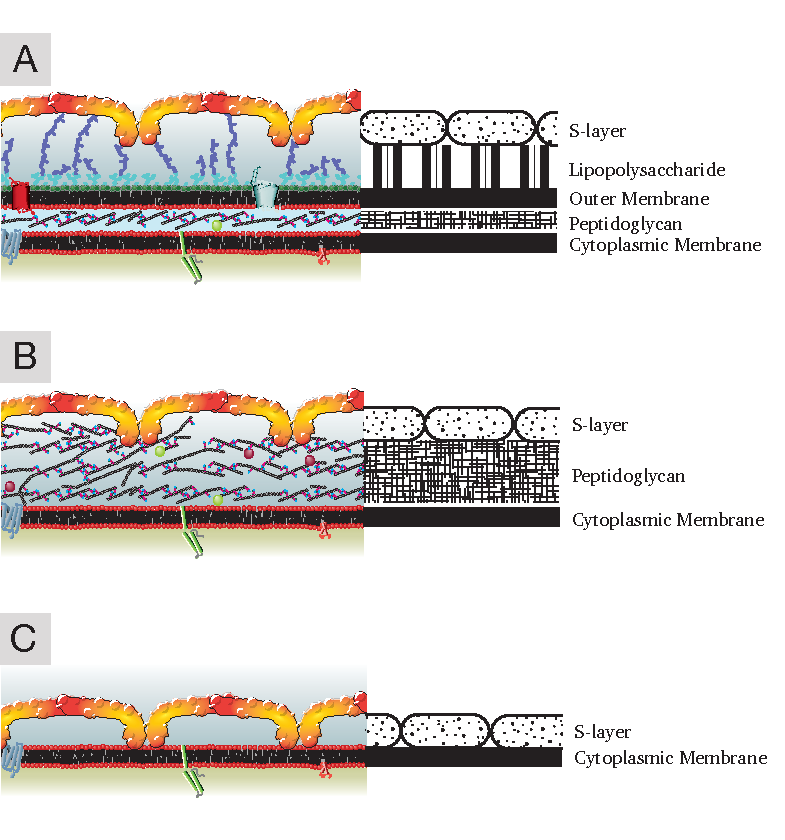
\includegraphics[]{intro/img/celwalls.pdf}
                \end{center}
                \caption[Cross-sectional diagrams of \ac{S-layer} containing cell envelopes]{Cross-sectional diagrams of the cell envelopes of (\textbf{A}) Gram negative bacteria, (\textbf{B}) Gram positive bacteria, and (\textbf{C}) archaebacteria. In all known cases the \ac{S-layer} sits on the extreme outer surface of the cell. (This diagram was inspired by Fig. 1 from \fullcite{sleytr1983crystalline})}
                \label{fig:cellwalls}
        \end{figure}

            Examples of bacteria with oblique \acs{S-layer} are \textit{Bacillus stearothermophilus} NRS2004$/$3a\upcite{messner1986characterization} and \textit{Lactobacillus brevis}\upcite[.]{masuda1980reassembly}
            Examples of bacteria with rectangular \acs{S-layer} are \textit{Corynebacterium diphtheriae}\upcite{kawata1972extracellular} and \textit{Aeromonas salmonicidae} A450\upcite[.]{ishiguro1981loss}
            An example of a bacterium with a triagonal \ac{S-layer} is \textit{Sulfolobus acidocaldarius}\upcite[.]{weiss1974subunit}
            Examples of bacteria with hexagonal \acs{S-layer} are \textit{Bacillus anthracis}\upcite{holt1969comparative} and \textit{Caulobacter crescentus}\upcite[.]{smit1981periodic}

        \begin{figure}[htb] % S-layer symmetries
                \begin{center}
                    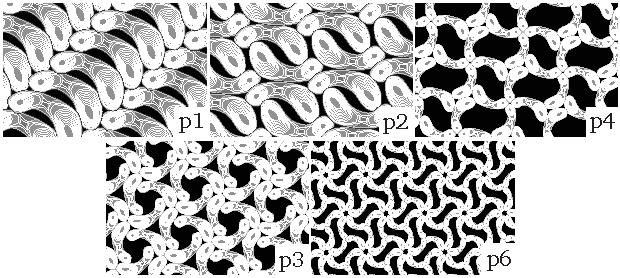
\includegraphics[]{intro/img/symmetries.pdf}
                \end{center}
                \caption[A simple overview of \ac{S-layer} symmetries]{A simple overview of \ac{S-layer} symmetries. p1 and p2 are oblique symmetries. 
                p4 is a rectangular symmetry.  
                p3  is a triagonal symmetry. 
                p6 is a hexagonal symmetry.}
                \label{fig:symmetries}
        \end{figure}


    % subsection s_layer_structure (end)

    \section{History of S-layers} % (fold)
    \label{sec:history_of_s_layers}
       
       % \begin{comment}  % Notes on history
       %      Notes on history of S-layers:
       %          - first seen
       %          - first cloned
       %          - first crystallised

       %      First (always) seen by EM

       %      First seen in Spirillum
       % \end{comment}

        \begin{figure}[p] % First S-layer
                \begin{center}
                    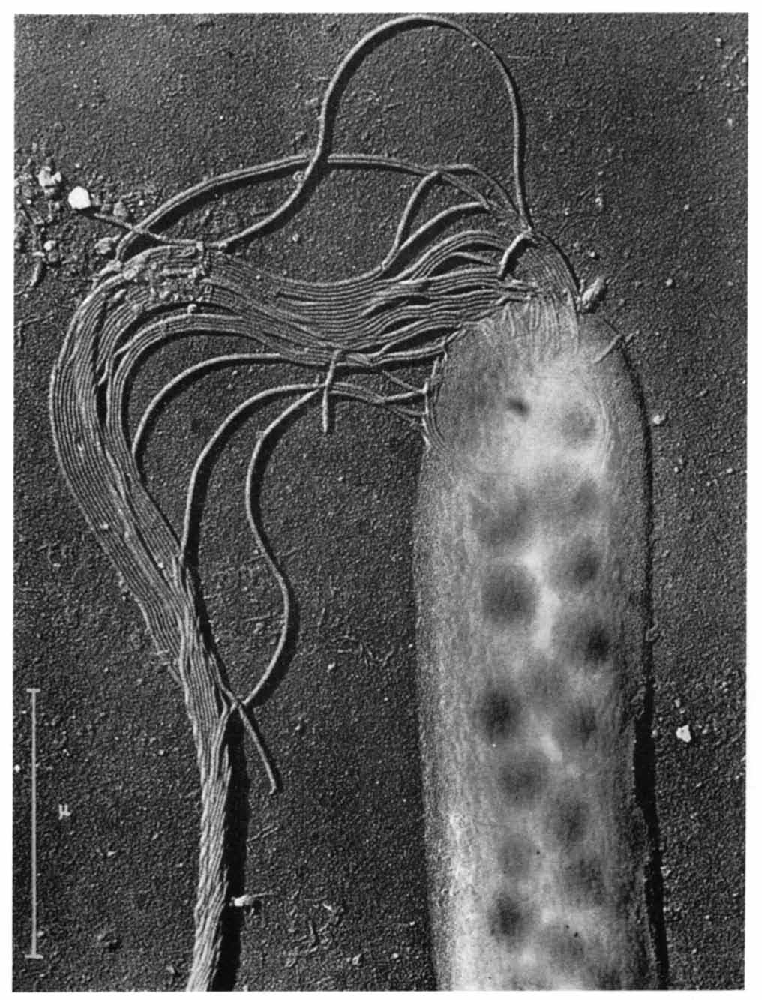
\includegraphics[]{intro/img/firstslayer.pdf}
                \end{center}
                \caption[The first published image of a \ac{S-layer}]{The first published image of a \ac{S-layer}. The hexagonal \ac{S-layer} on the surface of the bacterium --- probably \textit{Spirillum} sp. --- is visible along the edges of the cell body (centre right). The scale bar denotes one micrometre. (This image is Fig. 1 from \fullcite{firstslayer}, reused with full permission from the publisher, Elsevier.)}
                \label{fig:firstslayer}
        \end{figure}
    % section history_of_s_layers (end)
% section paracrystalline_protein_surface_layers (end)

\endinput

Any text after an \endinput is ignored.
You could put scraps here or things in progress.


%    2. Main body
% Generally recommended to put each chapter into a separate file
%% The following is a directive for TeXShop to indicate the main file
%!TEX root = ../MJThesis.tex
\acresetall

\chapter{The core and O-polysaccharide structure of the \textit{Caulobacter crescentus} lipopolysaccharide}
\label{ch:lps}
\begin{epigraph}
  \emph{``And so, progressively, the veil behind which Nature has so carefully concealed her secrets
    is being lifted where the carbohydrates are concerned.''} ---~H.\,Emil Fischer, 1902 Nobel
  lecture\\ My great-great-great-great-great-great-great-grand adviser.
\end{epigraph}
\section{Introduction} % (fold)
\label{sec:lps_introduction} 
\lettrine[lines=2]{C}{aulobacter crescentus} (\acs{caulobacter}) is an aquatic alphaproteobacterium
well known for a stalked, crescent cell morphology, asymmetric cell division, and a
\ac{S-layer}. \caulobacter is a widely studied model organism for cell development and
differentiation; despite this, the structure of its \ac{LPS} has not previously been fully
determined.

Interest in the \ac{LPS} of \caulobacter is focused on its immunological
profile\upcite{caulobacterlipida} and its structural role as an anchor for the
self-assembled, para-crystalline \ac{S-layer}\upcite[.]{walker94} The \ac{LPS}
of \caulobacter possesses a much reduced immunogenic activity, most likely due
to its lipid A structure, which is significantly different from that of
\ac{LPS} from enteric bacteria. The lipid A structure has been
reported\upcite[;]{caulobacterlipida} it is a unique molecule containing a
di-diaminoglucose backbone (instead of di-glucosamine) and two galacturonate
moieties that replace the canonical phosphates that are on each end of the
disaccharide in most lipid A molecules. The \caulobacter \ac{S-layer}
non-covalently attaches to the \ac{OPS}\upcite[.]{walker94} However, the
\ac{OPS} structure has not been resolved. Genetic analyses have pointed
towards the unusual N-acetylperosamine being a major
component\upcite[.]{awramgenes} A notable feature of this O-antigen is that it
exists completely hidden beneath the \ac{S-layer}, inaccessible to the
environment\upcite[.]{walker94} Carbohydrate structures from non-pathogenic
bacterial \ac{LPS} are rarely studied and an \ac{LPS} that is sequestered
beneath an \ac{S-layer} is not represented in the literature.
 
In the present study our data has determined the core \ac{OS} structure from
\caulobacter CB15 NA1000 (advancing an earlier report of core
composition\upcite{ravenscroftlps}), as well as the central backbone and
non-reducing ends of its \ac{OPS}. Unexpectedly, we identified a previously
unknown rhamnan polysaccharide. Along with previous reports on lipid
A\upcite{caulobacterlipida} and \ac{EPS}\upcite[,]{ravenscrofteps} we believe
that all the major carbohydrate structures in \caulobacter cell envelope have
now been solved.
% section introduction (end)

\section{Results} % (fold)
\label{sec:lps_results}
	\subsection{Characterization of whole \textsc{lps}} % (fold)
	\label{sub:characterisation_of_whole_lps}
		%% %^Write
  \begin{figure}[htb]
    \begin{center}
      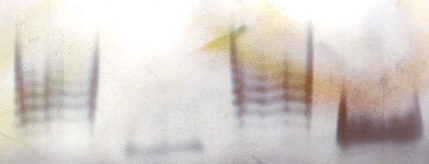
\includegraphics[width=0.3\textwidth]{lps_chapter/img/lpssilverstain.jpg}
    \end{center}
    \caption[Visual comparison of \ecoli O122 \ac{LPS} and \caulobacter \ac{LPS}]{Visual comparison
      of silver stained \ecoli O122 \ac{LPS} and \caulobacter \ac{LPS}. \ac{LPS} samples were run on
      a \ac{SDS-PAGE} and silver stained. Lanes 1 and 3 contain equal amounts of \ac{LPS} from
      \ecoli O122. Lanes 2 and 4 contain our isolated \ac{LPS} from \caulobacter. Lane 4 has twice
      the loaded amount compared to lane 2 to demonstrate that there are no minor, hidden
      bands. Notice the canonical `laddering' pattern of \ecoli\ \ac{LPS} and the distinctly
      singular band of \caulobacter\ \ac{LPS}.}
    \label{fig:lpssilverstain}
  \end{figure}

  \begin{figure}[htp]
    \begin{center}
      \includegraphics[]{lps_chapter/img/lpsvisuals.pdf}
    \end{center}
    \caption[Four different visualisations of \caulobacter\ \ac{LPS}]{Four different visualisations
      of \caulobacter\ \ac{LPS}. \textbf{A}. Western blot with rabbit anti-\ac{OPS} serum used as
      the primary probe. \textbf{B}. Far-western blot with RsaA \del 277--784 used as the primary
      probe and rabbit anti-RsaA serum used as the secondary probe. \textbf{C.} Schiff stained
      \ac{SDS-PAGE}. \textbf{D}. Silver stained \ac{SDS-PAGE}. The smooth-\ac{LPS} (\ie containing a
      complete \ac{OPS}) runs as a single band at roughly the equivalent rate of a 50 kDa protein
      and is visible in all lanes. The faint band visible at 30 kDa in the western blot (A) is of
      unknown source. The faint 30 kDa band is not seen in by far western (B), Schiff stain (C), or
      silver stain (D).}
    \label{fig:lpsvisuals}
  \end{figure}

  \begin{figure}[htb]
    \begin{center}
      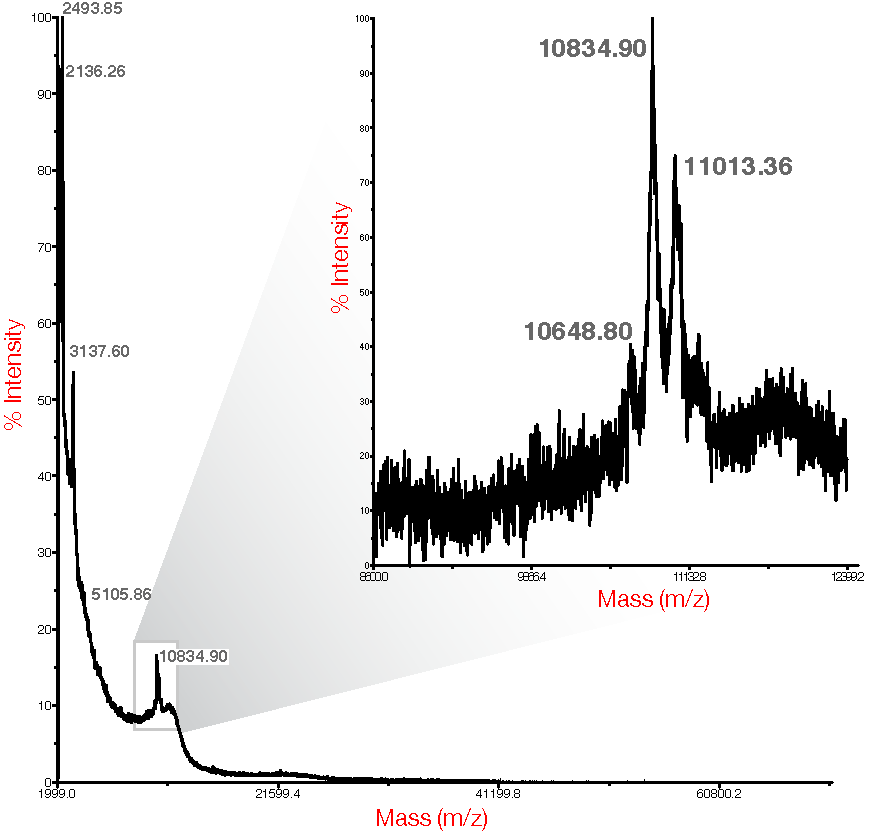
\includegraphics[]{lps_chapter/img/malditof.pdf}
    \end{center}
    \caption[\Ac{MALDI-TOF} analysis of intact, whole \ac{LPS} from \caulobacter]{\ac{MALDI-TOF}
      analysis of intact, whole \ac{LPS} from \caulobacter. The insert highlights the peaks
      attributed to \ac{LPS}. The major \ac{LPS} peak is labelled 10834.90 m/z}
    \label{fig:lpsmalditof}
  \end{figure}
	% subsection characterisation_of_whole_lps (end)

	\subsection{Initial assessment and component analysis} % (fold)
	\label{sub:initial_assessment_and_component_analysis}

  The \ac{PS} was released from the \ac{LPS} by hydrolysis with acetic acid. \textsuperscript{1}H
  \ac{NMR} spectrum of the \ac{PS} (\cref{fig:lpsfig1})) contained a large number of partially
  overlapping signals of various intensities in the anomeric region. It was obviously not a regular
  polymer with well-defined repeating units. Attempts to separate this material by anion-exchange
  chromatography led to the isolation of a number of fractions from neutral to slightly retained,
  but all of them had virtually identical \ac{NMR} spectra. Methylation of the polysaccharide led to
  the identification of 3- and 3,4-substituted mannopyranose, terminal glucopyranose (derived from
  side-chain 3-O-MeGlc), terminal, 3-, 4-, and 2,4-substituted rhamnopyranose, 3-substituted PerNAc,
  and an unidentified derivative resembling methylated PerN that eluted between dimethylhexose
  derivatives and 3-substituted PerNAc. To identify the position of the methyl groups in naturally
  methylated monosaccharides, methylation was conducted with \ce{CD3I}. This confirmed the
  identification of tetramethylglucitol as originating from 3-O-MeGlc, but did not identify any
  other naturally methylated monosaccharides, visible in \ac{NMR} spectra. An unknown derivative
  received two deuterated methyl groups.

  \begin{figure}[ph] %% 1D NMR Spectra
    \begin{center}
      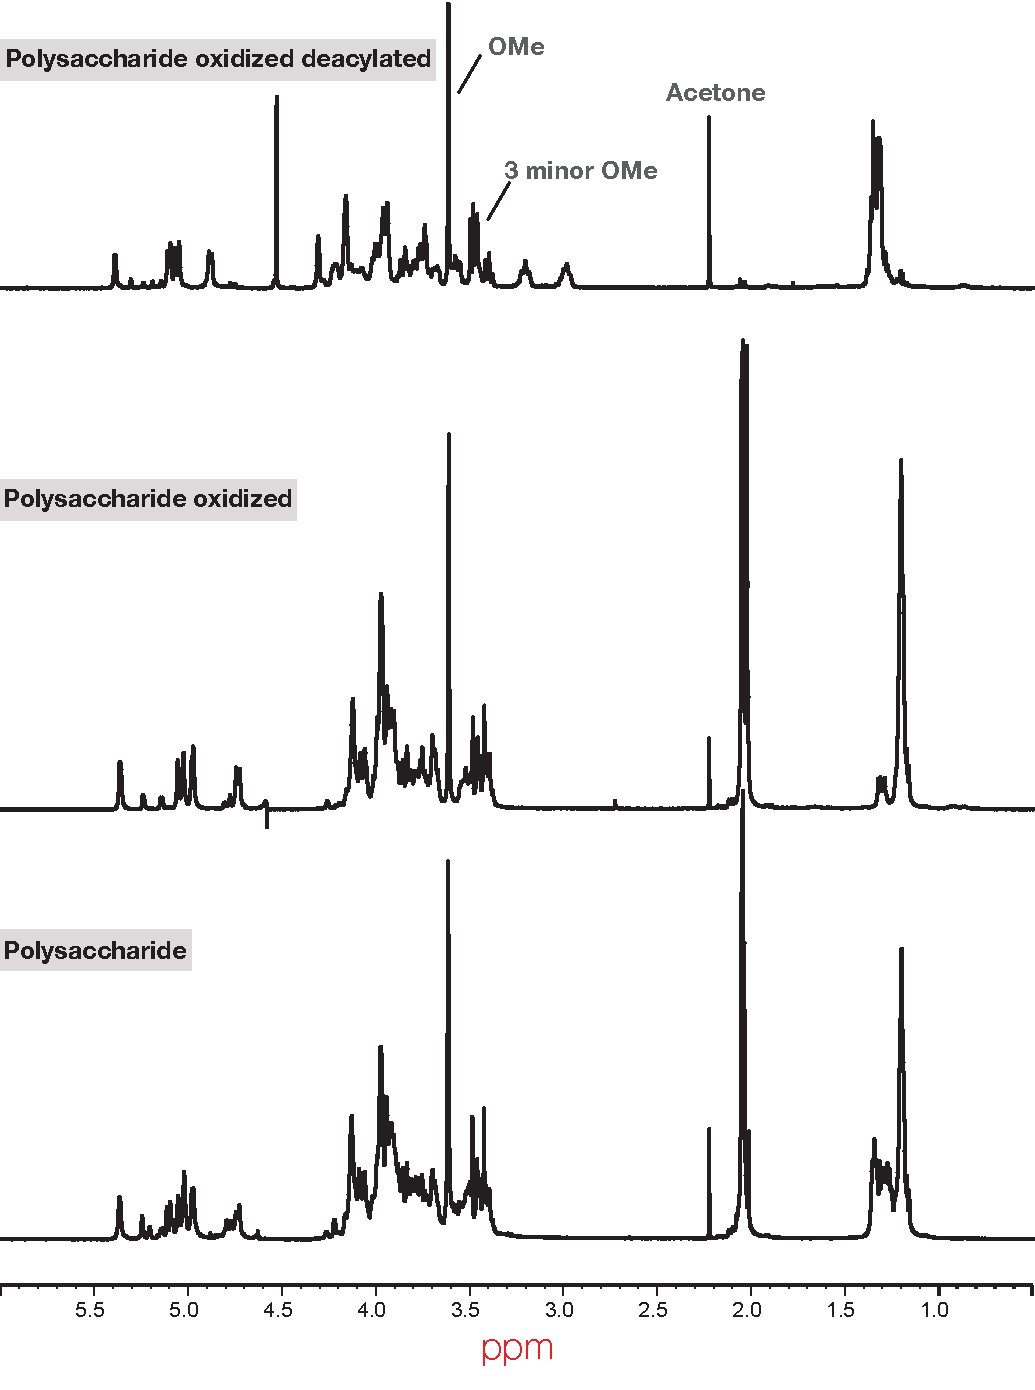
\includegraphics[height=0.9\textheight]{lps_chapter/img/lpsfig1.pdf}
    \end{center}
    \caption[\textsuperscript{1}H \ac{NMR} spectra of \caulobacter{} \ac{OPS}]{\textsuperscript{1}H
      \ac{NMR} spectra of the intact \caulobacter{} \ac{OPS} (bottom trace), double oxidized
      polysaccharide (middle trace) and N-deacylated double oxidized polysaccharide (upper trace).}
    \label{fig:lpsfig1}
  \end{figure}
	% subsection initial_assessment_and_component_analysis (end)

  \subsection{Identification of similar glycan structures by RsaA binidng} \label{sec:ident-simil-glyc}
  
  A service available at \ac{cfg} Core H at Emory University is glycan array screening\upcite[.]{blixt2004printed, alvarez2006identification} Fluorescently labeled lectins can be screened over an microarray of 465 known glycan structures commonly found in mammals. The array can be used to identify targets of known carbohydrate-binding proteins, such as RsaA. We hoped that RsaA may bind a glycan on the array and that the structure of that carbohydrate may inform us on the structure of the \ac{OPS} from \caulobacter. Due to our initial component analysis, knew that our \ac{OPS} differed significantly from any of the glycans in the array, at least compositionally (\vpageref{sub:initial_assessment_and_component_analysis}). RsaA (specifically RsaA \del 277--784) was found to not measurably bind any of the glycan structures found on the array. 

	\subsection{O-antigen structure determination (\textsc{ps}1)} % (fold)
	\label{sub:o_antigen_structure_determination_ps1_}

  A set of 2D spectra [\ac{gCOSY}, \ac{TOCSY}, \ac{NOESY},
  \textsuperscript{1}H-\textsuperscript{13}C \ac{gHSQC}, \ac{gHMBC}] was obtained for the
  \ac{PS}. There were many (more than 20) lines of correlations from the anomeric signals. Later,
  after the analysis of \ac{PS} degradation products, most of them could be assigned to particular
  structures (\cref{fig:lpsops,fig:lpsends,fig:lpsrhamnan}). Polysaccharide heterogeneity was not
  caused by random acetylation, but \ac{PS} contained 4 methyl groups (one major and 3
  minor). Monosaccharide analysis revealed L-Rha, D-Man, D-PerN (perosamine, 4-aminodeoxyrhamnose),
  and 3-O-MeGlc. Other methylated monosaccharides were not identified by \ac{GC-MS} as alditol
  acetates, possibly due to low content or degradation during hydrolysis. The \ac{GC-MS} data is
  presented in \cref{fig:monosaccharide_analysis}.

  \begin{figure}[htb] %% monosaccharides
    \begin{center}
      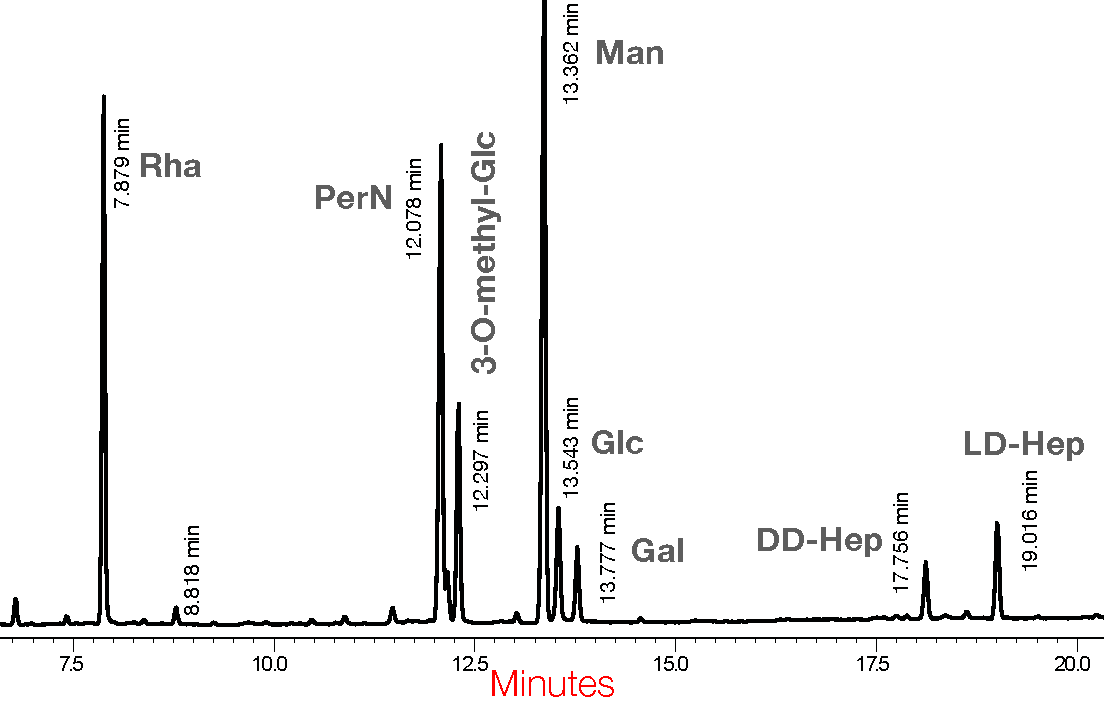
\includegraphics[width=\textwidth]{lps_chapter/img/lps_monosaccharides.pdf}
    \end{center}
    \caption[Monosaccharide analysis of \ac{LPS}]{Monosaccharide analysis of \caulobacter\
      \ac{LPS}. Alditol acetates derivatives of the \ac{LPS} component monosaccharides were
      separated and identified by \ac{GC-MS}. The protocol used is described on
      \cpageref{sub:monosaccharide_analysis}.}
    \label{fig:monosaccharide_analysis}
  \end{figure}

		In an attempt to simplify the structure, \ac{PS} was oxidized with \ce{NaIO4}, reduced with
    \ce{NaBD4}, hydrolysed with 2\% \ce{AcOH}, and the products were separated on a Biogel P6 column
    to give a polymer and an \ac{OS}, \ac{OS}1. Analysis of \ac{OS}1 will be described below. For
    some reason not all of the rhamnan was oxidized, and some of its signals persisted in the
    spectra of the remaining polymer (without side-chain Rha F). To remove the rest of it, the
    oxidation was repeated to produce \ac{PS}1. Spectra still contained some signals of minor
    components, analysed later. Assignment of the spectra of the non-oxidisable polymer \ac{PS}1 was
    difficult due to complete or partial overlap of the H-2,3,4,5 signals of PerNAc. To improve
    signal spread, \ac{PS}1 was deacylated with 4 M \ce{NaOH}. At this point the major polymer
    became positively charged and an attempt was made to separate it from the minor components using
    cation-exchange chromatography. However, all material was eluted together at high salt
    concentration, thus indicating that all components were chemically bound together. Assignment of
    the spectra (\cref{fig:lps2dnmr}, \cref{tbl:lpsops}) became possible at this stage due to better
    signal spread (H-4 signals of PerN moved to high field due to deacylation) and the sequence
    shown on \cref{fig:lpsops} was proposed. Spectra contained the signals of two
    $\beta$-mannopyranose, $\alpha$-3-O-MeGlc, and two -Per4N. The following interresidual \ac{NOE}
    and \ac{HMBC} correlations were used to determine the sequence: R1:L3, L1:Z3, Z1:Q3, Q1:W3,
    W1:X3, A1:X4. \Ac{PS}1 had trisaccharide repeating units composed of $\beta$-mannose and two
    $\alpha$-PerNAc residues, and every second repeating unit carried a side branch of 3-O-MeGlc. It
    seems that side-chains were present quite regularly at each second trisaccharide repeat of the
    main chain, because \ac{NOE} correlations were observed between the repeating units with and
    without 3-O-MeGlc, and not between units of the same structure. Thus altogether, the repeating
    unit contained seven monosaccharides.

		\begin{figure}[H]
			\begin{center}
				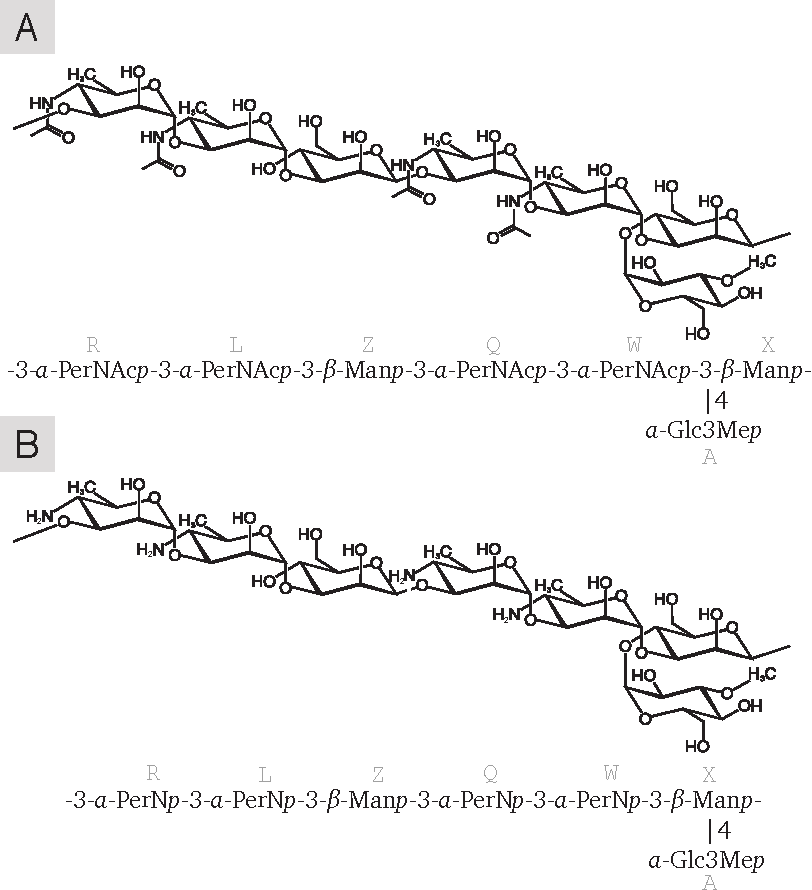
\includegraphics[]{lps_chapter/img/lpsops.pdf}
			\end{center}
			\caption[The structure of the \caulobacter \ac{OPS}]{The structure
            of the \caulobacter \ac{OPS}. \textbf{A.} The intact repeating unit,
            \ac{PS}1. \textbf{B.} The deacylated product of \ac{PS}1.}
			\label{fig:lpsops}
		\end{figure}

		\begin{figure}[H]
			\begin{center}
				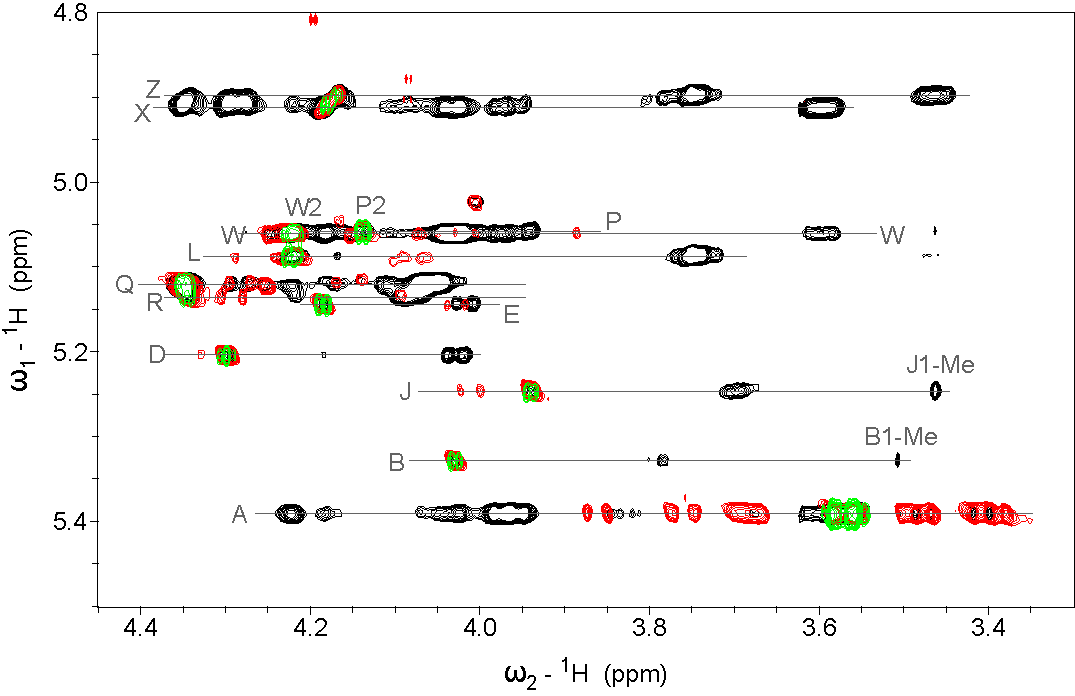
\includegraphics[width=0.9\textwidth]{lps_chapter/img/lpsfig3.pdf}
			\end{center}
			\caption[2D \ac{NMR} of \caulobacter{} \ac{PS}1]{Overlap of \ac{COSY} (green), \ac{TOCSY}
        (red) and \ac{ROESY} (black) correlations from anomeric protons of double oxidized
        deacylated \caulobacter{} \ac{PS}1.}
			\label{fig:lps2dnmr}
		\end{figure}
		\begin{table}[hp] % LPS OPS
			\centering
			\caption[\Ac{NMR} data for \caulobacter \ac{PS}1]{\Ac{NMR} data for \caulobacter \ac{PS}1 (40\cel) and deacylated \ac{PS}1 (50\cel). Me at 3.62/61.3 ppm.}
			\label{tbl:lpsops}
			\begin{tabular}{@{}rccccccc@{}}
				\toprule
				\multicolumn{8}{c}{PS1} \\ \midrule
     &   & 1     & 2    & 3    & 4    & 5    & 6 \\ \midrule
				\multirow{2}{*}{PerNAc R}      & H & 4.97  & 3.98 & 4.13 & 3.92 & 3.91 & 1.21 \\
     & C & 103.3 & 68.2 & 75.5 & 52.4 & 69.4 & 18.0 \\
				\multirow{2}{*}{PerNAc Q}      & H & 4.98  & 3.97 & 4.11 & 3.92 & 3.91 & 1.21 \\
     & C & 103.3 & 68.2 & 75.5 & 52.4 & 69.4 & 18.0 \\
				\multirow{2}{*}{PerNAc L}      & H & 5.05  & 4.12 & 3.99 & 3.98 & 3.98 & 1.21 \\
     & C & 103.3 & 70.4 & 78.2 & 53.0 & 69.4 & 18.0 \\
				\multirow{2}{*}{PerNAc W}      & H & 5.02  & 4.12 & 3.96 & 3.98 & 3.98 & 1.21 \\
     & C & 104.0 & 70.4 & 77.8 & 53.0 & 69.4 & 18.0 \\
				\multirow{2}{*}{$\beta$-Man X} & H & 4.74  & 4.09 & 3.98 & 3.90 & 3.54 & 3.80; 3.96 \\
     & C & 97.8  & 72.1 & 85.4 & 72.1 & 75.8 & 62.6 \\
				\multirow{2}{*}{$\beta$-Man Z} & H & 4.72  & 4.06 & 3.70 & 3.68 & 3.41 & 3.77; 3.96 \\
     & C & 98.2  & 71.9 & 82.3 & 67.2 & 77.3 & 62.4 \\
				\multirow{2}{*}{Glc3Me A}      & H & 5.36  & 3.51 & 3.40 & 3.44 & 3.68 & 3.75; 3.85 \\
     & C & 100.0 & 72.2 & 84.1 & 70.1 & 74.1 & 61.6 \\ \midrule
				\multicolumn{8}{c}{Deacylated PS1} \\ \midrule
				\multirow{2}{*}{PerN R}        & H & 5.13  & 4.34 & 4.29 & 3.30 & 4.18 & 1.38 \\
     & C & 103.5 & 67.4 & 75.0 & 53.4 & 67.8 & 18.0 \\
				\multirow{2}{*}{PerN Q}        & H & 5.11  & 4.34 & 4.29 & 3.30 & 4.18 & 1.38 \\
     & C & 103.5 & 67.4 & 75.0 & 53.4 & 67.8 & 18.0 \\
				\multirow{2}{*}{PerN L}        & H & 5.08  & 4.22 & 4.06 & 3.11 & 4.09 & 1.35 \\
     & C & 103.9 & 69.9 & 79.9 & 53.6 & 69.5 & 18.0 \\
				\multirow{2}{*}{PerN W}        & H & 5.06  & 4.22 & 4.06 & 3.11 & 4.09 & 1.35 \\
     & C & 103.9 & 69.9 & 79.9 & 53.6 & 69.5 & 18.0 \\
				\multirow{2}{*}{$\beta$-Man X} & H & 4.91  & 4.18 & 4.03 & 3.96 & 3.59 & 3.83; 3.96 \\
     & C & 98.0  & 71.7 & 85.0 & 71.7 & 75.9 & 62.1 \\
				\multirow{2}{*}{$\beta$-Man Z} & H & 4.90  & 4.18 & 3.75 & 3.75 & 3.46 & 3.83; 3.96 \\
     & C & 98.0  & 71.7 & 82.0 & 67.0 & 77.4 & 62.1 \\
				\multirow{2}{*}{Glc3Me A}      & H & 5.39  & 3.57 & 3.40 & 3.48 & 3.68 & 3.76; 3.86 \\
     & C & 100.2 & 72.2 & 84.0 & 70.0 & 74.1 & 61.7 \\ \bottomrule
			\end{tabular}
		\end{table}
	% subsection o_antigen_structure_determination_ps1_ (end)
  
	\subsection{Minor component determination} % (fold)
	\label{sub:minor_component_determination}

  \ac{PS} and \ac{PS}1 spectra contained signals of minor components, which could not be removed by
  chromatography, as described above. They probably represented the non-reducing ends of the major
  chain, \ac{PS}1 (\cref{fig:lpsends}). The minor components contained methylated Rha (2-O-Me-Rha
  residue J and 2,3-Me$_2$-PerN residue B). The position of the methyl groups were found from
  \ac{HMBC} correlations between protons of methyl groups and carbon atoms bearing OMe groups, which
  all were well visible and did not overlap with other signals due to their low field
  position. Thus, two independent structural fragments, 1 and 2, were found and are shown in
  \cref{fig:lpsends}. Mannose residues Z' and Z" at the non-reducing ends of these fragments were
  further linked to PerN residues, indistinguishable from the PerN of the main chain. PerN residue D
  had upfield shifted C-2 and downfield shifted C-3 signals (\cref{tbl:lpsends})), which have not
  been explained. It appears that its O-3 was phosphorylated, producing typical phosphorylation
  signal shifts and broadening of the H-3 signal, but \textsuperscript{1}H-\textsuperscript{31}P
  \ac{HMQC} \ac{NMR} spectrum showed no signals, possibly due to the low abundance of this
  residue. Possibly Rha residues inserted in the structure resembling \ac{PS}1 represented the
  attachment point of the rhamnan (\ac{PS}2) to \ac{PS}1, if they were linked together.

		 \begin{figure}[htb]
		 	\begin{center}
		 		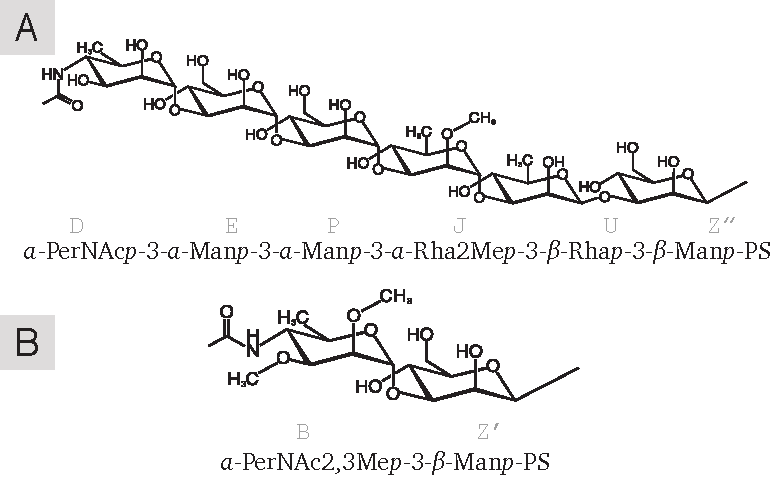
\includegraphics[]{lps_chapter/img/lpsends.pdf}
		 	\end{center}
		 	\caption[The structure of minor component, the end caps of the \ac{OPS}.]{The structure of minor component, the end caps of the \ac{OPS}. \textbf{A.} Fragment 1. \textbf{B.} Fragment 2.}
		 	\label{fig:lpsends}
		 \end{figure}

		 \begin{table}[htb]
			 \centering
			 \caption[\Ac{NMR} data for the minor components of the double oxidized non-deacylated \ac{PS}]{\ac{NMR} data for the minor components of the double oxidized non-deacylated \ac{PS} (50\cel). Methyl group signals: B2: 3.48/59.5; B3: 3.42/57.9; J2: 3.45/59.6 ppm (H/C)}
			 \label{tbl:lpsends}
			 \begin{tabular}{@{}rccccccc@{}}
				 \toprule
         &   & 1     & 2    & 3    & 4    & 5    & 6 \\ \midrule
				 \multirow{2}{*}{PerN2,3Me B}       & H & 5.25  & 3.96 & 3.71 & 3.81 & 3.91 & 1.17 \\
         & C & 100.2 & 76.2 & 78.2 & 53.2 & 69.5 & 18.0 \\
				 \multirow{2}{*}{$\alpha$-Rha2Me J} & H & 5.25  & 3.95 & 4.02 & 3.45 & 3.90 & 1.30 \\
         & C & 100.2 & 75.9 & 75.4 & 71.8 & 69.5 & 18.0 \\
				 \multirow{2}{*}{$\alpha$-PerN D}   & H & 5.14  & 4.27 & 4.20 & 3.95 & 3.97 & 1.23 \\
         & C & 100.1 & 67.4 & 75.2 & 52.2 & 69.4 & 18.0 \\
				 \multirow{2}{*}{$\alpha$-Man E}    & H & 5.13  & 4.17 & 3.99 & 3.75 & 3.84 & \\
         & C & 100.1 & 70.9 & 79.8 & 67.1 & 74.4 & \\
				 \multirow{2}{*}{$\alpha$-Man P}    & H & 5.05  & 4.14 & 4.00 & 3.85 & 3.96 & \\
         & C & 97.6  & 71.0 & 79.5 & 66.9 & 74.0 & \\
				 \multirow{2}{*}{$\beta$-Rha U}     & H & 4.78  & 4.16 & 3.69 & 3.48 & 3.44 & 1.32 \\
         & C & 100.9 & 71.8 & 82.0 & 72.4 & 73.1 & 18.0 \\
				 \multirow{2}{*}{$\beta$-Man Z"}    & H & 4.72  & 4.06 & 3.75 & 3.75 & 3.46 & 3.83; 3.96 \\
         & C & 98.2  & 71.9 & 86.0 & 67.0 & 77.4 & 62.1 \\
				 \multirow{2}{*}{$\beta$-Man Z'}    & H & 4.72  & 4.06 & 3.73 & 3.75 & 3.46 & 3.83; 3.96 \\
         & C & 98.2  & 71.9 & 82.3 & 67.0 & 77.4 & 62.1 \\ \bottomrule
			 \end{tabular}
		 \end{table} %
	% subsection minor_component_determination (end)

	\subsection{Rhamnan polysaccharide determination (\textsc{ps}2)} % (fold)
	\label{sub:rhamnan_polysaccharide_determination_ps2_}

  Periodate oxidation of the \ac{PS} produced an \ac{OS}1, which was analyzed by \ac{NMR} and its
  structure, as shown on \cref{fig:lpsrhamnan}, was determined using standard 2D \ac{NMR}
  methods. Signal assignment is shown in the \cref{tbl:lpsrhamnan}. It contained three
  rhamnopyranose units and 4-deoxy-1-deutero-erythritol, produced by the oxidation-reduction of
  4-substituted rhamnose. Formation of this oligosaccharide could be explained by oxidation of the
  side chain Rha F and 4-substituted Rha G in the \ac{PS}1 (letter labels for monosaccharides were
  given using anomeric signals in the whole \ac{PS} spectra starting from low-field). The unoxidized
  4-substituted residue T in the oligosaccharide originally carried side-chain Rha F at position
  2. Knowing the \ac{OS}1 structure the signals of a corresponding polymer (\ac{PS}2) were
  identified in the spectra of the whole \ac{PS}, and are given in the \cref{tbl:lpsrhamnan}.

		\begin{figure}[htb]
			\begin{center}
				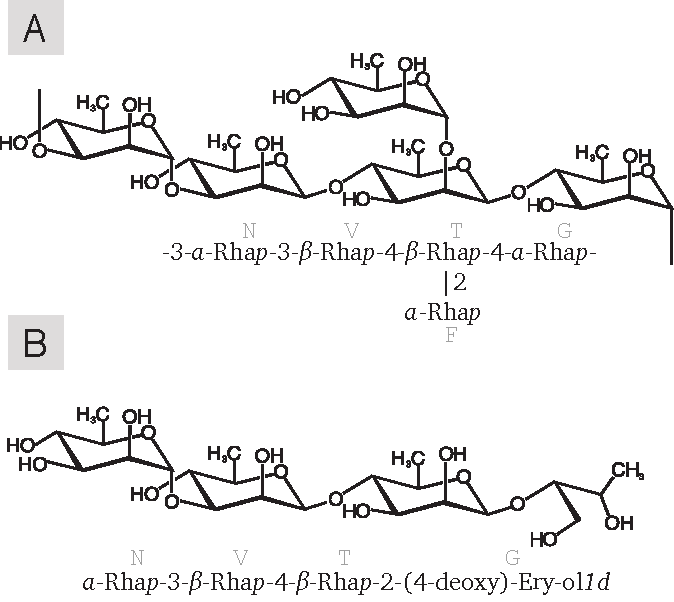
\includegraphics[]{lps_chapter/img/lpsrhamnan.pdf}
			\end{center}
			\caption[The structure of the \caulobacter rhamnan.]{The structure of the \caulobacter rhamnan. \textbf{A.} the intact rhamnan, \ac{PS}2. \textbf{B.} the oxidised rhamnan product, \ac{OS}1.}
			\label{fig:lpsrhamnan}
		\end{figure}

		\begin{table}[ht]
			\centering
			\caption[\Ac{NMR} data for \caulobacter  \ac{PS}2 and its \ce{NaIO4} oxidation product \ac{OS}1]{\ac{NMR} data for \caulobacter  \ac{PS}2 and its \ce{NaIO4} oxidation product \ac{OS}1 (40\cel).}
			\label{tbl:lpsrhamnan}
			\begin{tabular}{@{}rccccccc@{}}
				\toprule
				                                     &   & 1          & 2    & 3    & 4    & 5    & 6 \\ \midrule
				\multirow{2}{*}{$\alpha$-Rha N, OS1} & H & 5.04       & 4.07 & 3.85 & 3.47 & 3.85 & 1.30 \\
				                                     & C & 103.1      & 71.1 & 71.1 & 72.9 & 69.9 & 17.6 \\
				\multirow{2}{*}{$\alpha$-Rha N, PS}  & H & 5.02       & 4.02 & 3.79 & 3.45 & 3.72 & 1.28 \\
				                                     & C & 103.0      & 71.5 & 78.8 & 73.3 & 70.4 & 17.5 \\
				\multirow{2}{*}{$\beta$-Rha T, OS1}  & H & 4.78       & 4.13 & 3.71 & 3.54 & 3.53 & 1.33 \\
				                                     & C & 100.7      & 71.1 & 72.3 & 83.4 & 71.7 & 17.5 \\
				\multirow{2}{*}{$\beta$-Rha T, PS}   & H & 4.79       & 4.22 & 3.82 & 3.62 & 3.61 & 1.36 \\
				                                     & C & 101.7      & 76.7 & 73.5 & 83.4 & 73.2 & 17.5 \\
				\multirow{2}{*}{$\beta$-Rha V, OS1}  & H & 4.75       & 4.12 & 3.67 & 3.49 & 3.49 & 1.34 \\
				                                     & C & 101.1      & 71.4 & 81.3 & 71.9 & 72.9 & 17.5 \\
				\multirow{2}{*}{$\beta$-Rha V, PS}   & H & 4.77       & 4.13 & 3.66 & 3.66 & 3.50 & 1.35 \\
				                                     & C & 101.4      & 71.2 & 81.7 & 67.2 & 73.3 & 17.5 \\
				\multirow{2}{*}{X (ox. G), OS1}      & H & 3.69; 3.71 & 3.75 & 3.99 & 1.20 &      & \\
				                                     & C & 61.8       & 84.8 & 67.7 & 18.0 &      & \\
				\multirow{2}{*}{$\alpha$-Rha G, PS}  & H & 5.10       & 4.13 & 3.94 & 3.58 & 3.90 & 1.35 \\
				                                     & C & 103.1      & 71.5 & 70.3 & 84.5 &      & 17.5 \\
				\multirow{2}{*}{$\alpha$-Rha F, PS}  & H & 5.11       & 4.09 & 3.87 & 3.45 & 4.07 & 1.27 \\
				                                     & C & 102.4      & 72.1 & 71.3 & 73.3 &      & 17.5 \\ \bottomrule
			\end{tabular} %% LPS Rhamnan
		\end{table}
	% subsection rhamnan_polysaccharide_determination_ps2_ (end)

	\subsection{Core oligosaccharide determination} % (fold)
	\label{sub:core_oligosaccharide_determination}

  The core oligosaccharide of the \caulobacter{} \ac{LPS} isolated after \ce{AcOH} hydrolysis
  contained one non-degraded Kdo, two LD-Hep, one DD-Hep, mannose, galactose, and glucuronic acid in
  pyranose form. 2D \ac{NMR} analysis led to the structure shown on \cref{fig:lpscore} (\ac{NMR}
  assignments are in \cref{tbl:lpstable4}, the \ac{HSQC} spectrum is in \cref{fig:lpscorenmr}). The
  sequence followed from the observed \ac{NOE}: E1:C5,C7,F5; F1:E2; G1:F3; H1:C7,E2; K1:C4;
  L1:K4. Correlation E1:C7 is always observed in the $\alpha$-Hep-5-Kdo fragment. E1:F5 was due to
  the $\alpha$-Man-2-Hep linkage. H1E2 indicates spatial proximity of the residues E and H, linked
  to the same Kdo C. All expected transglycoside correlations were observed in \ac{HMBC} spectrum,
  together with intra-ring correlations H-1:C-3 and H-1:C-5 for all $\alpha$-pyranoses. Methylation
  analysis revealed terminal DD-Hep, terminal and 2-substituted LD-Hep, 3-substituted Man and
  terminal Gal. The structure agreed with mass spectral data, \ac{ESI} \ac{MS} in negative ion mode,
  [M-H]\textsuperscript{-} = 1314.9, [M-2H]/2\textsuperscript{-} = 656.7, calculated exact mass Hex
  x 2 + Hep x 3 + HexA x 1 + Kdo x 1 = 1314.4 Da.

		\begin{figure}[htb]
			\begin{center}
				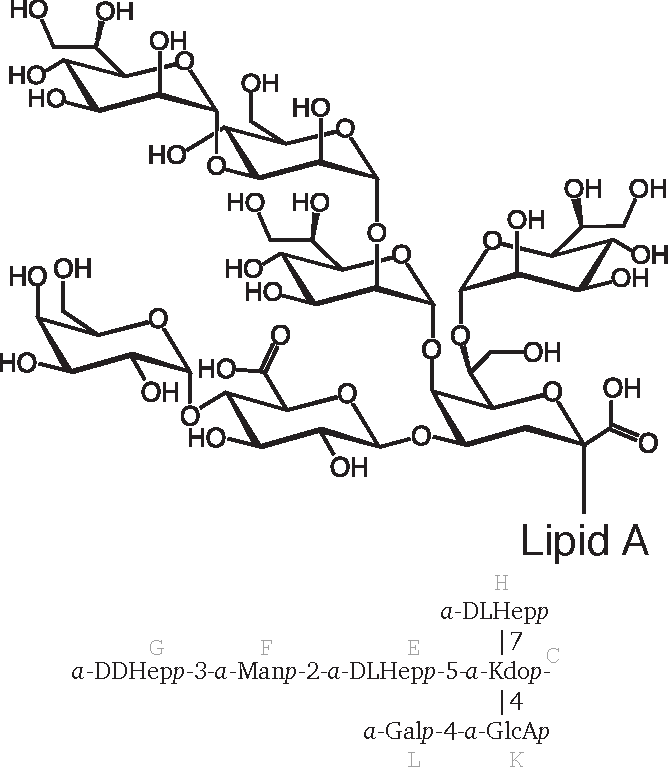
\includegraphics[]{lps_chapter/img/lpscore.pdf}
			\end{center}
			\caption{The structure of the \caulobacter core \ac{OS}.}
			\label{fig:lpscore}
		\end{figure}

		\begin{table}[htb]
			\centering
			\caption[\Ac{NMR} data for the core oligosaccharide]{\ac{NMR} data for the core oligosaccharide (25\cel).}
			\label{tbl:lpstable4}
			\begin{tabular}{@{}rccccccccc@{}}
        \toprule
        &   & 1     & 2    & 3          & 4    & 5    & 6          & 7          & 8 \\ \midrule
        \multirow{2}{*}{Kdo C}   & H &       &      & 2.05; 2.35 & 4.23 & 4.28 & 4.09       & 3.91       & 3.81; 3.93 \\
        & C &       & 98.2 & 34.7       & 74.9 & 74.2 & 71.0       & 79.2       & 61.5 \\
        \multirow{2}{*}{DLHep E} & H & 5.24  & 3.85 & 4.12       & 3.89 & 3.88 & 4.04       & 3.73; 3.73 & \\
        & C & 101.1 & 80.2 & 71.1       & 67.3 & 74.1 & 70.0       & 63.9       & \\
        \multirow{2}{*}{Man F}   & H & 5.03  & 4.30 & 4.00       & 3.79 & 3.80 & 3.80; 3.91 &            & \\
        & C & 103.7 & 70.6 & 78.1       & 67.5 & 74.5 & 62.0       &            & \\
        \multirow{2}{*}{DDHep G} & H & 5.15  & 4.05 & 3.86       & 3.77 & 3.84 & 4.06       & 3.76; 3.84 & \\
        & C & 103.1 & 71.0 & 71.8       & 68.7 & 74.5 & 72.9       & 62.9       & \\
        \multirow{2}{*}{DLHep H} & H & 5.07  & 4.14 & 3.89       & 3.89 & 3.80 & 4.10       & 3.79; 3.81 & \\
        & C & 102.7 & 73.7 & 71.8       & 67.3 & 73.2 & 70.2       & 64.9       & \\
        \multirow{2}{*}{GlcA K}  & H & 5.22  & 3.66 & 4.00       & 3.99 & 4.15 &            &            & \\
        & C & 98.8  & 72.4 & 74.9       & 73.6 &      &            &            & \\
        \multirow{2}{*}{Gal L}   & H & 5.49  & 3.80 & 3.85       & 3.99 & 3.94 & 3.69; 3.69 &            & \\
        & C & 99.9  & 69.7 & 70.3       & 70.0 & 71.8 & 61.6       &            & \\ \bottomrule
			\end{tabular}%LPS table 4
		\end{table}

		\begin{figure}[htb]
			\begin{center}
				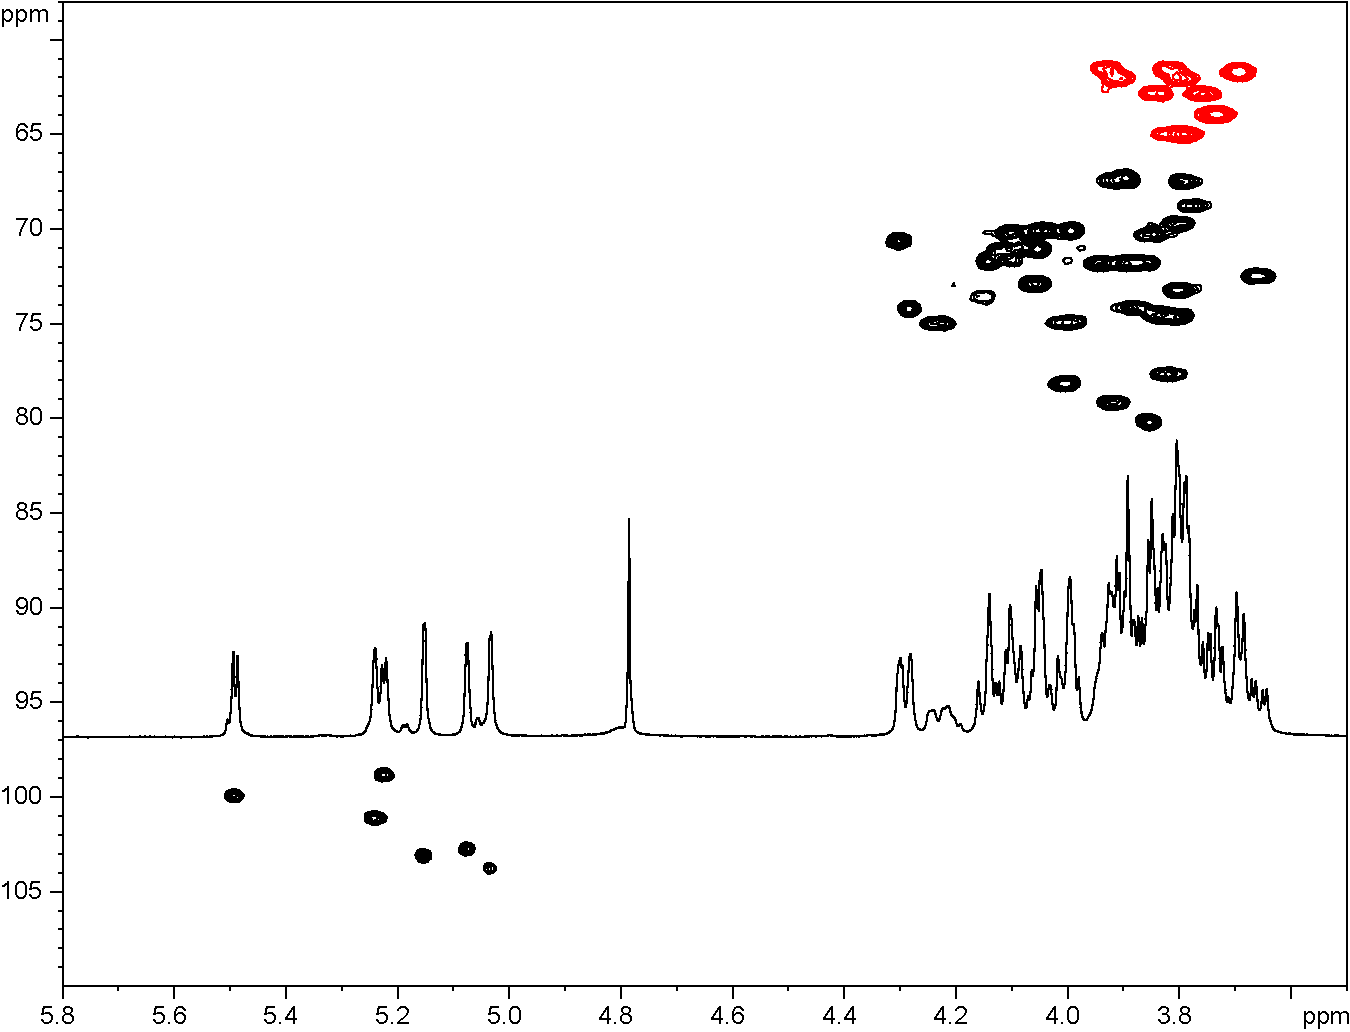
\includegraphics[width=\textwidth]{lps_chapter/img/lpsfig4.pdf}
			\end{center}
			\caption{Fragment of \textsuperscript{1}H-\textsuperscript{13}C \ac{HSQC} spectrum of the core.}
			\label{fig:lpscorenmr}	
		\end{figure}
    % subsection core_oligosaccharide_determination (end)
    \subsection{Cellular response to \textit{C. crescentus} LPS}\label{sec:cell-resp-text}

   \begin{figure}[htb]
  	\begin{center}
   		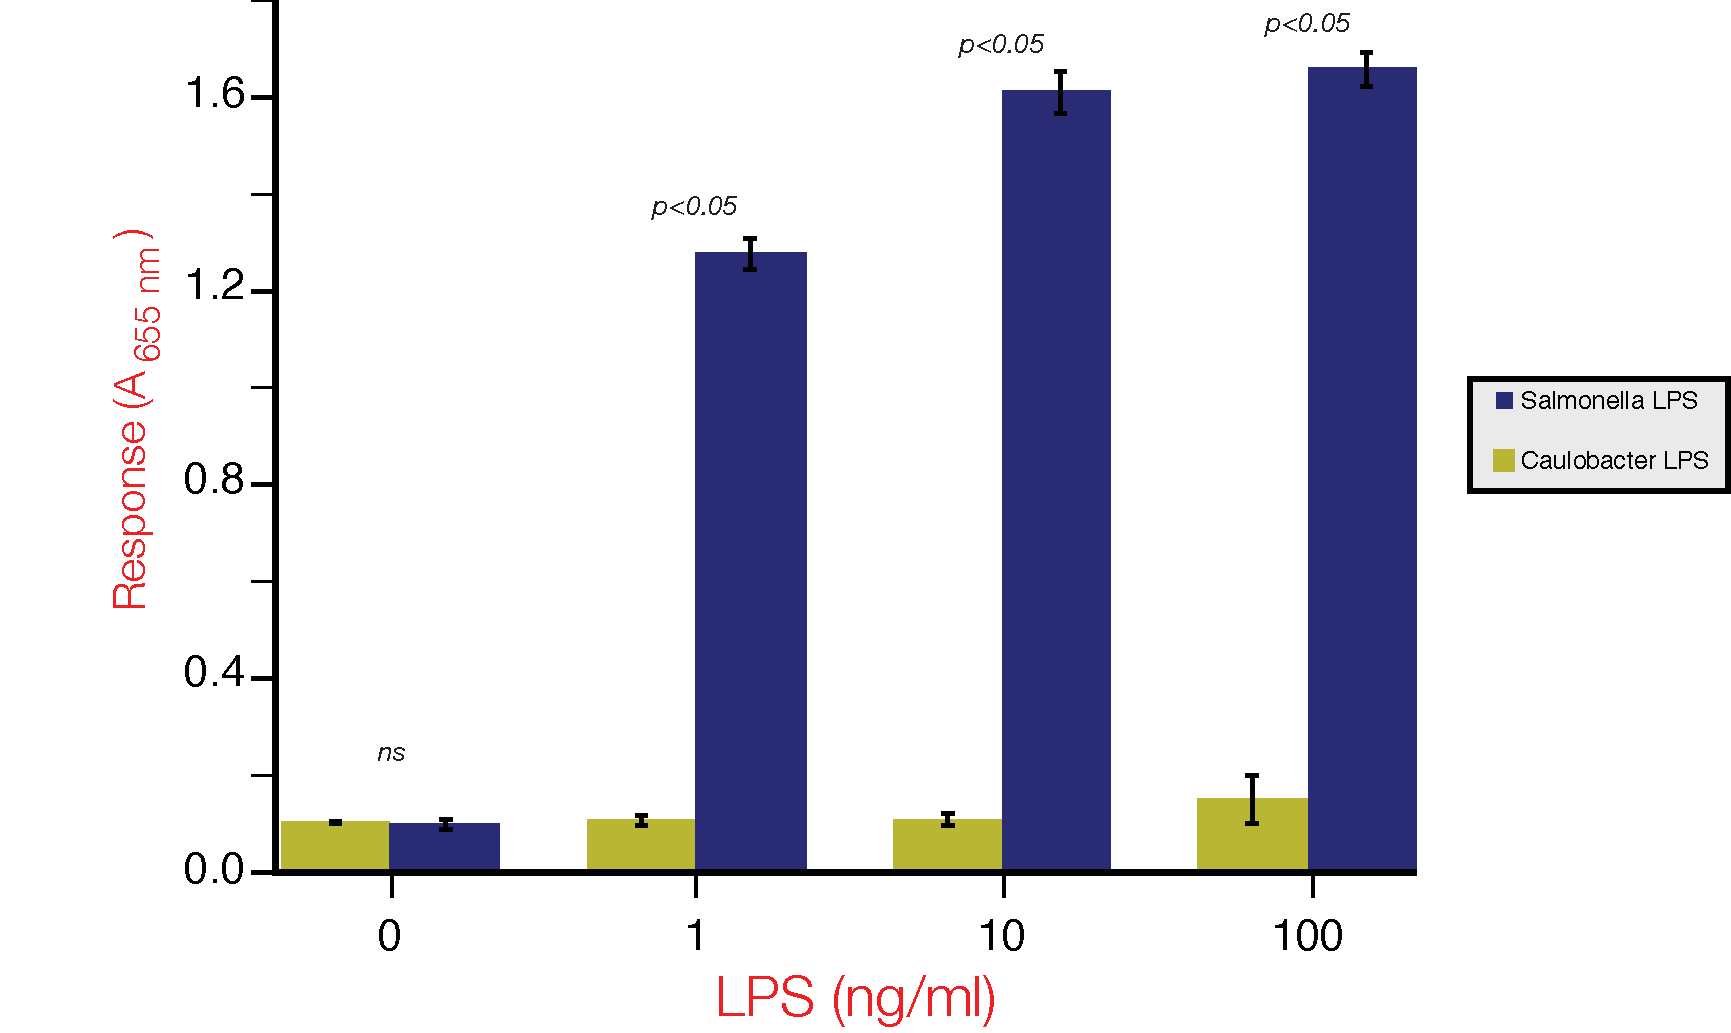
\includegraphics[width=\textwidth]{lps_chapter/img/NFkBAssay.pdf}
   	\end{center}
   	\caption[NF$\kappa$B Assay for cellular activation by LPS]{
	   	\textbf{TITLE} TEXT % Add adescription!
   	}
   	\label{fig:nfkbassay}
\end{figure}    
% section results (end)


\section{Methods} % (fold)
\label{sec:lps_methods}

	\subsection{Bacterial strain construction and growth conditions} % (fold)
	\label{sub:bacterial_strain_construction_and_growth_conditions}

  The strain used for the preparation of \ac{LPS} was JS1025, a derivative of \caulobacter CB15
  NA1000. The salient features are that it has an engineered amber mutation in \textit{rsaA} leading
  to the loss of the \ac{S-layer} and the gene CCNA\_00471 has been inactivated by a partial
  deletion. CCNA\_00471 encodes a putative GDP-L-fucose synthase\upcite[.]{na1000genome} The
  knockout (\del 471) confers a deficiency in an \ac{EPS} that was previously found to contain
  L-fucose\upcite[.]{ravenscrofteps} CCNA\_00471 was disrupted in the same manner as previously in
  JS4038\upcite[,]{hivmicrobicide2} except the starting strain used here was
  JS1023\upcite[.]{slayercryo}
		
  Cells were grown to mid-to-late log phase (\od = 0.9) in M16HIGG defined medium at 30\cel in 2.8
  \si{\litre} Fernbach flasks containing 1250 \millilitre of medium, shaking at 100 rpm. M16HIGG is
  a modification of M6HIGG medium\upcite[,]{smitpilin81} containing 0.31\% glucose, 0.09\%
  glutamate, 1.25 \si{\milli\meter} sodium phosphate, 3.1 \si{\milli\meter} imidazole, 0.05\%
  ammonium chloride, and 0.5\% modified Hutner's Mineral Base\upcite[.]{hutners}
	% subsection bacterial_strain_construction_and_growth_conditions (end)

	\subsection{\textsc{lps} isolation} % (fold)
	\label{sub:LPS_isolation}
  \ac{LPS} was isolated from the cells via disrupting the outer membrane by chelation.  The the
  negative charges in Gram negative bacterial \ac{LPS} are stabilised and bridged by available
  divalent cations (\ie{} \ce{Ca^2+} and \ce{Mg^2+}). Lieve first noted in 1965\upcite{leive65} that
  one can strip the counter ions from the outer membrane to disrupt it and cause it to shed into the
  medium. We chose a chelation strategy because we found it easy to scale up, it didn't require
  noxious organic solvents, and because our lab's first attempt to isolate and analyse \caulobacter\
  \ac{LPS}\upcite{ravenscroftlps} using the Darveau extraction method\upcite{darveauprocedure} only
  resulted in the isolation of core+lipidA (rough \ac{LPS}).

  The protocol we used was a modification of the procedure reported by Walker
  \etal\!\upcite{walker94} Cells were centrifuged at 12 400 x g for 10 min. The pellets were
  suspended with distilled water and recentrifuged. These pellets were resuspended in 1/10 original
  culture volume in \ac{PBS}\upcite{maniatis} amended with 35 \si{\milli\meter} \ac{EDTA}, agitated
  at room temperature for 10 min and then centrifuged at 15 300 x g for 15 min. The supernatant was
  retrieved and re-centrifuged, as before, to ensure clarity and then dialysed against 5
  \si{\milli\meter} \ce{MgCl2}. DNase and RNase were added to final concentrations of 10
  \si{\micro\gram\per\milli\litre} and 100 \si{\micro\gram\per\milli\litre}\!, respectively, and
  incubated at 37\cel for 2 h. Proteinase K was added to a final concentration of 0.3 \mgperml and
  the preparation was incubated at 50\cel overnight. The sample was then ultracentrifuged at 184 000
  x g for 3 h. Glassy pellets formed which were suspended in distilled water to 1/100 original
  culture volume. A Bligh-Dyer extraction was performed to reduce contaminating
  lipids\upcite[.]{blighdyer}
	% subsection \ac{LPS}_isolation (end)

	\subsection{Bligh Dyer Extraction} % (fold)
	\label{sub:bligh_dyer_extraction}
  A Bligh Dyer extraction was performed on all \ac{LPS} preparations to reduce the presence of
  contaminating lipids. The extraction was performed as first published\upcite[.]{blighdyer} In
  short, to one volume of aqueous \ac{LPS} sample, 3.75 volumes of chloroform/methanol (1:2 v/v) was
  added and the sample was vortexed for 30 seconds. 1.25 volumes of chloroform was added and the
  sample was vortexed again for 30 seconds. 1.25 volumes of water were added and the sample was
  vortexed a final time for 30 seconds. This mixture was then centrifuged at 15 300 x g for 10
  min. After centrifugation, the mixture separated in to two phases, a lower organic phase and an
  upper aqueous phase. The \ac{LPS} partitions into the aqueous phase, while other lipids partition
  into the organic phase. The aqueous phase was retrieved and kept.
	% subsection bligh_dyer_extraction (end)

	\subsection{Silver stain and gel electrophoresis} % (fold)
	\label{sub:gel_electrophoresis}

  Discontinuous \ac{SDS-PAGE} was performed with a 13\% separating gel\upcite[.]{laemmli} Detection
  of \ac{LPS} was done by periodate oxidation and silver staining as described by Zhu
  \etal\!\upcite{improvedsilverstain} The silver stain protocol is a newer technique that uses
  vitamin C (ascorbic acid) in place of formaldehyde in traditional \ac{LPS}
  stains\upcite[.]{tsai1982sensitive} Table \ref{tbl:silver} give the details of the silver stain
  procedure.

		% Please add the following required packages to your document preamble:
		% \usepackage{booktabs}
		\begin{table}[ht]  % Silver stain table
			\centering
			\caption{\Ac{LPS} silver stain procedure}
			\label{tbl:silver}
			\begin{tabular}{@{}rcl@{}}
				\toprule
				\textbf{Step} & \textbf{Solution}                                                           & \textbf{Time} \\ \midrule
				Oxidation     & 30\% EtOH, 10\% HOAc, 0.7\% periodic acid                                   & 10 	min     \\
				Rinse         & d\ce{H2O}                                                                   & 5 min x2   \\
				Silver        & 0.2\% \ce{AgNO3}                                                            & 5 min      \\
				Rinse         & d\ce{H2O}                                                                   & 20 sec x2  \\
				Develop       & 3\% \ce{NaCO3}, 0.04\% \ce{Na2S2O3}, 0.02\% ascorbic acid, 0.05\% \ce{NaOH} & 8 min      \\
				Stop          & 10\% HOAc                                                                   & 1 min \\ \bottomrule
			\end{tabular}
		\end{table}
	% subsection gel_electrophoresis (end)
    \subsection{Preparation of RsaA \del 277--784 probe} \label{sec:preparation-rsaa-del}
    
    The plasmid, p4BRsaA\del 277--784, was extant in our laboratory from the work of Wade Bingle. In short, various versions of rsaA were engineered to have \textit{Bam}HI sites at locations throughout the gene\upcite[.]{bingle1997linker} The \textit{Bam}HI--\textit{Hin}DIII fragment from a version of rsaA with a \textit{Bam}HI site at the 831 bp from the start codon was replaced with a \textit{Bam}HI--\textit{Hin}DIII fragment from a version of rsaA with a \textit{Bam}HI site at the 2352 bp position. In effect this made a rsaA gene missing 1521 bp from the center, corresponding to amino acids 277--784 within the resulting protein. This `internally truncated' gene was then moved into the context of our expression vector `p4B'\upcite[]{lau2010analysis} as a \textit{Eco}RI--\textit{Hin}DIII fragment.
    
    \subsection{Periodic acid-Schiff Stain} % (fold)
    \label{sub:schiff_stain}
		
    Periodic   acid-Schiff   stain   was   performed   on  \ac{LPS}   samples   that   were   run   on
    \ac{SDS-PAGE}. Schiff stain is analogous to silver  stain in that it identifies carbohydrates that
    are first oxidised with periodic acid.

    The staining procedure starts by soaking the gel on a slow shaker in 0.7\% periodic acid in
    distilled water for 15 min. The gel is then rinsed in distilled water and placed in Schiff reagent
    and shaken slowly for 15 min. The gel is then washed in distilled water for 5 min, at which time
    pink bands should appear that are correspond to polysaccharides/\ac{LPS} in the gel.

    The protocol to prepare Schiff's reagent started by dissolving 5 \si{\gram} of basic fuchsin in
    900 \millilitre of boiling distilled water. Once dissolved the fuchsin solution was removed from
    heat and allowed to cool for a few minutes, then 100 \millilitre of 1 \si{\molar}\ \ce{HCl} was
    slowly added. After the solution was allowed to cool to room temperature, 10 \si{\gram} of
    \ce{K2S2O5} was added. This solution was thoughly mixed, then incubated in the fume hood
    overnight. The next day, a few spoonfuls of activated charcoal were added to the Schiff reagent to
    decolourize the solution. The solution was stired and then filtered through Watman paper \# 1. The
    now clear Schiff stain solution was ready to use. It had a sulfurous smell and would stain nearly
    any surface it was spilled on a vibrant pink colour. A test for Schiff reagent activity would be
    to add a few drops of Schiff reagent to 5 \millilitre of formaldehyde in a test tube. The mixture
    should instantly turn a bright pink colour, indicating activity.
    % subsection schiff_stain (end)

      \subsection{\textsc{nmr} spectroscopy} % (fold)
      \label{sub:nmr_spectroscopy}

      \ac{NMR} experiments were carried out on a Varian INOVA 600 \si{\mega\hertz}
      (\textsuperscript{1}H) spectrometer with 5 \si{\milli\meter} gradient probe at 25--50\cel with
      acetone internal reference (2.225 ppm for \textsuperscript{1}H and 31.45 ppm for
      \textsuperscript{13}C), using standard pulse sequences \ac{gCOSY}, \ac{TOCSY}(mixing time 120
      \si{\milli\second}), \ac{ROESY} (mixing time 300 \si{\milli\second}), \ac{gHSQC}, and
      \ac{gHMBC}(100 \si{\milli\second} long range transfer delay), \ac{HMQC} for
      \textsuperscript{1}H-\textsuperscript{31}P correlation, J$_{HX}$ set to 10
      \si{\hertz}. Acquisition time was kept at 0.8--1 sec for H-H correlations and 0.25 sec for
      \ac{HSQC}. 256 increments were acquired for t$_1$ in all 2D spectra, except 512 for \ac{gCOSY}.
      % subsection nmr_spectroscopy (end)

      \subsection{\textsc{lps} Chromatography} % (fold)
      \label{sub:chromatography}

      Gel chromatography was performed on a Sephadex G-15 column (1.5 x 60 \si{\centi\meter}) or a
      Bio-gel P6 column (2.5 x 60 \si{\centi\meter}) in pyridine-acetic acid buffer (4 \millilitre:10
      \millilitre:1 \si{\litre} water), and monitored by refractive index detector (Gilson). Anion
      exchange chromatography was done on an Hitrap Q column (2x5 \millilitre size, Amersham), with
      \ac{UV} monitoring at 220 nm in a linear gradient of \ce{NaCl} (0--1 M, 1 h) at the 3
      \si{\milli\litre\per\minute}. Fractions of 1 min were collected and additionally tested for
      carbohydrates, by spotting on an \ce{SiO2} \ac{TLC} plate, dipping them in 5\% \ce{H2SO4} in
      \ce{EtOH} and heating with a heat-gun. All fractions of interest were dried in a Savant drying
      centrifuge and \textsuperscript{1}H spectra were recorded for each fraction without desalting. For
      2D \ac{NMR}, desalting was performed on a Sephadex G15 column.
      % subsection chromatography (end)x`'

      \subsection{Monosaccharide analysis} % (fold)
      \label{sub:monosaccharide_analysis}

      Samples with added inositol standard were hydrolysed with 3 M \ac{TFA} at 120\cel. Monosaccharides
      were converted to alditol acetates by conventional methods and identified by \ac{GC-MS} on a
      Varian Saturn 2000 instrument on a DB17 capillary column (30 m x 0.25 \si{\milli\meter} ID x 0.25
      \si{\micro\meter} film) with helium carrier gas, using a temperature gradient 170\cel (3
      min)--250\cel at 5\si{\degreeCelsius\per\minute}.
      % subsection monosaccharide_analysis (end)

      \subsection{Determination of absolute configurations of monosaccharides} % (fold)
      \label{sub:determination_of_absolute_configurations_of_monosaccharides}

      To the polysaccharide sample (0.2 \milligram) (R)-2-\ce{BuOH} (0.2 \millilitre) and acetyl
      chloride (0.02 \millilitre) were added at room temperature, heated at 90\cel for 2 h, dried by air
      stream, acetylated, analysed by \ac{GC-MS} as described above. Standards were prepared from
      monosaccharides of known configuration with (R)- and (S)-2-\ce{BuOH}.
      % subsection determination_of_absolute_configurations_of_monosaccharides (end)

      \subsection{Methylation analysis} % (fold)
      \label{sub:methylation_analysis}

      For the methylation analysis core sample (2 \milligram) was dephosphorylated with 50 \microlitre
      of 48\% \ce{HF} for 20 h at +10\cel, diluted with 2 \millilitre of ethanol, precipitate collected
      by centrifugation, washed with 2 \millilitre of ethanol, dried.

      Methylation was performed by Ciucanu-Kerek procedure\upcite[.]{ciucanufrancisc} 0.5 \milligram of
      the sample was dissolved in 0.5 \millilitre of dry DMSO with heating at 100\cel for 5-10 min until
      complete dissolution. Powdered \ce{NaOH} (about 50 \milligram) was added and the mixture was
      stirred for 30 min. 0.2 \millilitre of \ce{MeI} was added and the mixture was stirred for a
      subsequent 30 min. The sample was then flushed with air to remove the MeI and diluted to 10
      \millilitre with water. The sample was passed through a C18 Seppak cartridge, washed with 10
      \millilitre of water, and then the methylated compound was eluted with 5 \millilitre of
      methanol. The methylated product was hydrolysed with 3 M \ac{TFA} (120\cel, 3h), dried, reduced
      with \ce{NaBD4}, and the reagent destroyed with 0.5 \millilitre of 4 M \ce{HCl}. The solution was
      dried under a stream of air and dried twice more with the addition of \ce{MeOH} (1
      \millilitre). The sample was acetylated with 0.4 \millilitre{} \ce{Ac2O} and 0.4 \millilitre
      pyridine for 30 min at 100\cel. It was then dried and analysed by \ac{GC-MS}.
      % subsection methylation_analysis (end)

      \subsection{Periodate oxidation} % (fold)
      \label{sub:periodate_oxidation}

      \ac{PS} (10 \milligram) was dissolved in water (2 \millilitre). \ce{NaIO4} (20 \milligram) was
      added and the solution was incubated at room temperature for 24 h. Ethylene glycol (0.2
      \millilitre) and an excess \ce{NaBD4} were added. The solution was then kept for 1 h before being
      treated with 0.2 \millilitre of \ce{AcOH} and desalted on a Sephadex G-15 column. The product was
      hydrolysed with 2\% \ce{AcOH}, 2 h at 100\cel, and separated on a Sephadex G-50 column to give
      \ac{OS}1.
      % subsection periodate_oxidation (end)
      % section methods (end)

      \section{Discussion} % (fold)
      \label{sec:lps_discussion}

      The \ac{LPS} of \caulobacter has an unusually complicated structure with two different
      polysaccharides, irregular substituents, and unfavourable \ac{NMR} spectra. Presented data show
      structures of the core part, two polymers, and putative terminal structures. The polysaccharides
      could not be separated by size exclusion or anion-exchange chromatography and are probably linked
      together through the same core. The core of the \caulobacter{} \ac{LPS} has been studied previously
      and an initial assessment of its composition was made\upcite[,]{ravenscroftlps} but the complete
      structure had not been determined. The structure of the \ac{OPS} has not been studied before. In our
      view the polysaccharide structure of the \caulobacter{} \ac{LPS} represents one of the most
      complicated bacterial \ac{LPS} polysaccharide structures identified so far.

      The Kdo present in the \ac{LPS} core structure (see \cref{fig:lpscore}) has the typical
      substitutions at O-4 and O-5 of a manno-configured sugar and a negatively charged sugar,
      respectively\upcite[.]{brade99} It also has a rarely observed third substitution at O-7 with a
      heptose moiety. The Kdo O-7 position is known to be occupied by a galactose moiety in the core of
      \textit{Rhizobium leguminosarum} bv. Viciae VF39\upcite[,]{rhizobiumlps} and the secondary Kdo in
      the core oligosaccharide from \textit{Acinetobacter baumannii} ATCC 19606 has an O-7 substituted
      with a glucosamine\upcite[.]{acinetobacterlps}

      In the traditional model \ac{LPS} occupies the outer leaflet of the outer membrane of a
      Gram-negative bacterium, and so (excepting the presence of cell associated \ac{EPS}) is the
      outermost layer of the cell. For \caulobacter, however, \ac{LPS} is the penultimate barrier below
      the protein \ac{S-layer}. The \caulobacter{} \ac{OPS} serves as the anchor for the S-layer and is
      likely not accessible to the environment\upcite[.]{walker94} The carbohydrates found in the \ac{OPS}
      are particularly hydrophobic, marked by the abundance of deoxy-sugars, acetyl groups, and methyl
      groups. This hydrophobicity is possibly a result of particular sugars needed for \ac{S-layer}
      anchoring, as these carbohydrate structures likely evolved as the cognate ligands for the
      \ac{S-layer} protein, RsaA. The distance between the \ac{S-layer} and the outer membrane is about
      17--19 nm\upcite[.]{dipm} It is possible the hydrophobicity aids in packing the polysaccharides
      between the S-layer and the \ac{LPS}. Further determination of RsaA's structure should help
      illuminate the interaction between the S-layer and \ac{OPS}.

      Knowledge of the structure of \caulobacter{} \ac{OPS} and \ac{LPS} will facilitate the determination
      and characterization of their biosynthetic enzymes and mutant variants. Already, the enzymes
      LpxI\upcite{lpxi} and GDP-L-perosamine acetylase\upcite{perosmineacetyltransferase} from
      \caulobacter have been characterized. One uncharacterised enzyme, WbqL, is necessary for proper
      \ac{OPS} synthesis and disruption of wbqL leads to the accumulation of truncated and S-layer
      anchoring deficient \ac{OPS} in the inner membrane and inhibits Crescentin-mediated cell
      curvature\upcite[.]{lpsinterferecrescentin} Many genes, such as wbqL, have been identified as
      essential for \ac{OPS} synthesis\upcite{awramgenes} but have not yet been characterized. Other
      genes, that must be essential for \ac{OPS} synthesis, have yet to be identified or characterized,
      such as the O-antigen polymerase and ligase.

      % --Should I increase the text about lpxI?--%

      The subunit-based repeating nature of \caulobacter{} \ac{OPS} suggests that a Wzy-dependent pathway
      synthesizes the polymer\upcite[.]{lpsreview02} The previous study that aimed to identify genes
      essential for \ac{OPS} did not identify many of the canonical genes in the Wzy-dependant
      pathway\upcite[,]{awramgenes} such as the O-unit transporter, Wzx, O-antigen polymerase, Wzy; the
      chain-length determinate protein, Wzz; and the O-antigen ligase, WaaL. Genes that have been
      annotated as putative O-antigen synthesis genes do appear in the sequenced genomes for \caulobacter
      CB15, but they have not been experimentally confirmed.

      An additional aspect to this \ac{LPS} it the fact that its O-antigen is of homogeneous length. While
      other \ac{LPS}s vary in size due to the number of O-antigen repeat groups, appearing as a laddering
      of bands by \ac{SDS-PAGE}, the \ac{LPS} from \caulobacter appears as a single
      band\upcite[.]{walker94} Initial \ac{MALDI-TOF} analysis of the entire \ac{LPS} indicates a size of
      about 10.8 kDa (see \cref{fig:lpsmalditof} on \cpageref{fig:lpsmalditof}).  After accounting for the
      solved structures for the lipid A and core regions, this suggests the \ac{LPS} contains
      approximately 5 repeats of the proposed heptameric O-antigen structure.  There is not currently a
      known mechanism for the regulation and synthesis of a strictly homogeneous length O-antigen. It is
      possible that this \ac{OPS} is synthesized via the \ac{ABC}-transporter-dependent
      pathway\upcite{lpsreview02} or another heretofore undiscovered mechanism. In any event it would seem
      that the transfer of a polysaccharide of this considerable size to the outer leaflet of the outer
      membrane is a remarkable feat for the bacterium.

%\include{model}
%\include{impl}
%\include{discussion}
%\include{conclusions}
%    3. Notes
%    4. Footnotes
%    5. Bibliography
% prints author names as small caps
\renewcommand{\mkbibnamefirst}[1]{\textsc{#1}}
\renewcommand{\mkbibnamelast}[1]{\textsc{#1}}
\renewcommand{\mkbibnameprefix}[1]{\textsc{#1}}
\renewcommand{\mkbibnameaffix}[1]{\textsc{#1}} 
\printbibliography[heading=bibintoc]

\appendix
%    6. Appendices (including copies of all required UBC Research
%       Ethics Board's Certificates of Approval)
%\include{reb-coa}	% pdfpages is useful here
\chapter*{Appendix}
% \section{The amino aid sequence of RsaA from \caulobacter}
\begin{figure}[htb]
  	\begin{center}
\label{app:rsaseq}
\texttt{\singlespacing\small\underline{MAYTTAQLVTAYTNANLGKAPDAATTLTLDAYATQTQTGGLSDAAALTNTLKLVNSTTAV}\hfill-60~~\\
\underline{AIQTYQFFTGVAPSAAGLDFLVDSTTNTNDLNDAYYSKFAQENRFINFSINLATGAGAGA}\hfill-120~\\
\underline{TAFAAAYTGVSYAQTVATAYDKIIGNAVATAAGVDVAAAVAFLSRQANIDYLTAFVRANT}\hfill-180~\\
\underline{PFTAAADIDLAVKAALIGTILNAATVSGIGGYATATAAMI}NDLSDGALSTDNAAGVNLFT\hfill-240~\\
AYPSSGVSGSTLSLTTGTDTLTGTANNDTFVAGEVAGAATLTVGDTLS\textbf{GGAGTDVLN}WVQ\hfill-300~\\
AAAVTALPTGVTISGIETMNVTSGAAITLNTSSGVTGLTALNTNTSGAAQTVTAGAGQNL\hfill-360~\\
TATTAAQAANNVAVDGGANVTVASTGVTSGTTTVGANSAASGTVSVSVANSSTTTTGAIA\hfill-420~\\
VTGGTAVTVAQTAGNAVNTTLTQADVTVTGNSSTTAVTVTQTAAATAGATVAGRVNGAVT\hfill-480~\\
ITDSAAASATTAGKIATVTLGSFGAATIDSSALTTVNLSGTGTSLGIGRGALTATPTANT\hfill-540~\\
LTLNVNGLTTTGAITDSEAAADDGFTTINIAGSTASSTIASLVAADATTLNISGDARVTI\hfill-600~\\
TSHTAAALTGITVTNSVGATLGAELATGLVFT\textbf{GGAGADSILL}GATTKAIVMGAGDDTVTV\hfill-660~\\
SSATLGAGGSVN\textbf{GGDGTDVLV}ANVNGSSFSADPAFGGFETLRVAGAAAQGSHNANGFTAL\hfill-720~\\
QLGATAGATTFTNVAVNVGLTVLAAPTGTTTVTLANATGTSDVFNLTLSSSAALAAGTVA\hfill-780~\\
LAGVETVNIAATDTNTTAHVDTLTLQATSAKSIVVTGNAGLNLTNTGNTAVTSFDASAVT\hfill-840~\\
GTGSAVTFVSANTTVGEVVTIR\textbf{GGAGADSLT}GSATANDTII\textbf{GGAGADTLV}YTGGTDTFT\textbf{G}\hfill-900~\\
\textbf{GTGADIFD}INAIGTSTAFVTITDAAVGDKLDLVGISTNGAIADGAFGAAVTLGAAATLAQ\hfill-960~\\
YLDAAAAGDGSGTSVAKWFQFGGDTYVVVDSSAGATFVSGADAVIKLTGLVTLTTSAFAT\hfill-1020\\
EVLTLA\hfill-1026\\
  }
   	\end{center}
   	\caption[RsaA, amino acid sequence]{
   The amino acid sequence of the \ac{S-layer} protein, RsaA from \caulobacter{} NA1000. GeneID:~\texttt{CCNA\_01059}. Ensembl Accession number: \texttt{ACL94524}. The encoding gene has the coordinates of 1 159 693 bp--1 162 773 bp on the forward strand of the \caulobacter chromosome. The underlined sequence corresponds to the amino acids 1--222, the section of the protein that was removed to generate a crystallizable C-terminal fragment. The bolded sequences are the \ac{rtx} motifs in RsaA. For the crystallization of RsaA, see \cref{ch:crystal} \cpageref{ch:crystal}.}
   	
\end{figure}   
% \section{The amino acid sequence of OmpW from \caulobacter}
\begin{figure}[htb]
  	\begin{center}
\label{app:ompwseq}
\texttt{\singlespacing\small  MKKLALSLVAFGALAAGAAQAQDFTPNAKGDLIVHARLTQVAPAKDAAILTAAGANSGLK\hfill-60~\\
AHVGNDIKPTLGFTYFLTDKVAVEAILGTTEHNIRAQGPGTDVLVHKTWVLPPVVTLQYH\hfill-120\\
PLPASQVSPYVGAGLNYMLFYSGKNKNGFTVKVDDGVGYALQAGVNIKMKNSWLVNADV\textbf{K}\hfill-180\\
KVYFSTDAKINGGALKAKVDLDPVVASIGLSRKF\hfill-214\\
  }
   	\end{center}
   	\caption[OmpW, amino acid sequence]{
   The amino acid sequence of the outer membrane channel, OmpW from \caulobacter NA1000. GeneID: \texttt{CCNA\_01475}. Ensembl Accession number: \texttt{ACL94940}. The encoding gene has the coordinates of 1 582 599 bp--1 583 243 bp on the forward strand of the \caulobacter chromosome. The bolded `K' is the location of the putative hydrophobic gate in \ecoli and \ac{pseudomonas}, where that residue encodes for a tryptophan; in \caulobacter that residue is a lysine. For our investigations into OmpW, see \cref{ch:porin} on \cpageref{ch:porin}}
\end{figure}   



\backmatter
%    7. Index
% See the makeindex package: the following page provides a quick overview
% <http://www.image.ufl.edu/help/latex/latex_indexes.shtml>


\end{document}
